%!TeX program = xelatex
\documentclass[12pt,hyperref,a4paper,UTF8]{ctexart}
\usepackage[sort&compress]{gbt7714} 
\usepackage{SJTUReport}
\usepackage{booktabs} % 三线表
\usepackage{siunitx}

\definecolor{c1}{HTML}{2752C9} 
%   listing代码环境设置
\usepackage{listings}
\usepackage{subfig}
\lstloadlanguages{bash}
\lstdefinestyle{bashstyle}{
backgroundcolor=\color{gray!5},
language=bash,
frameround=tftt,
frame=shadowbox,
keepspaces=true,
breaklines,
columns=spaceflexible,
escapeinside=``,
basicstyle=\ttfamily\small, % 基本文本设置,字体为teletype,大小为scriptsize
keywordstyle=[1]\color{c1}\bfseries,
keywordstyle=[2]\color{red!70!black},
keywordstyle=[3]\color{teal!70!white},
stringstyle=\color{lightgray},
showstringspaces=false,
commentstyle=\ttfamily\scriptsize\color{green!40!black},%注释文本设置,字体为sf,大小为smaller
tabsize=2,
morekeywords=[1]{ln, cp, git, mkdir, fm_shell, tee, v2lvs, echo,
                pt_shell, source},
morekeywords=[2]{snf, clone, add, push, commit, config, add,
                },
morekeywords=[3]{},
numbers=left, % 代码行数
numberstyle=\it\tiny\color{gray}, % 代码行数的数字字体设置
stepnumber=1,
rulesepcolor=\color{gray!30!white}
}

\lstloadlanguages{Verilog}
\lstdefinestyle{Verilogstyle}{
backgroundcolor=\color{gray!5},
language=Verilog,
frameround=tftt,
frame=shadowbox, 
keepspaces=true,
breaklines,
columns=spaceflexible,                   
basicstyle=\ttfamily\small, % 基本文本设置,字体为teletype,大小为scriptsize
keywordstyle=[1]\color{c1}\bfseries, 
keywordstyle=[2]\color{red!70!black},
keywordstyle=[3]\color{teal!70!white},
stringstyle=\color{purple},       
showstringspaces=false,
commentstyle=\ttfamily\scriptsize\color{green!40!black},%注释文本设置,字体为sf,大小为smaller
tabsize=2,
morekeywords=[2]{},
morekeywords=[3]{jpeg_top_tb, jpeg_top, UUT, jpeg_top_inst, jpeg_asic, PLBI8F},
numbers=left, % 代码行数
numberstyle=\it\tiny\color{gray}, % 代码行数的数字字体设置
stepnumber=1,
rulesepcolor=\color{gray!30!white}
}

\lstloadlanguages{tcl}
\lstdefinestyle{tclstyle}{
backgroundcolor=\color{gray!5},
language=tcl,
frameround=tftt,
frame=shadowbox, 
keepspaces=true,
breaklines,
columns=spaceflexible,                   
basicstyle=\ttfamily\small, % 基本文本设置,字体为teletype,大小为scriptsize
keywordstyle=[1]\color{c1}\bfseries, 
keywordstyle=[2]\color{red!70!black},
keywordstyle=[3]\color{teal!70!white},
stringstyle=\color{purple},       
showstringspaces=false,
commentstyle=\ttfamily\scriptsize\color{green!40!black},%注释文本设置,字体为sf,大小为smaller
tabsize=2,
morekeywords=[1]{vlib, vmap, vlog, vsim, add, run, create_clock, get_ports,
                    set_ideal_network, set_case_analysis, remove_from_collection,
                    get_pins, all_inputs, set_clock_uncertainty, set_driving_cell,
                    all_clocks, set_load, set_input_delay, set_output_delay,
                    all_outputs, load_of, formDefault, setFormField,
                    menuReload, auVerilogToCell, formButton, geOpenLib,
                    formOK, geOpenCell, axgLoadTDF, axgPlanner, formApply,
                    date, set_svf, read_verilog, sh, set_top, read_verilog,
                    read_db, lappend, current_design, link_design, set_min_library,
                    reset_design, read_parasitics, set_wire_load_mode, set_wire_load_model,
                    set_propagated_clock, report_clocks, set_drive, set_max_fanout,
                    set_false_path,  report_design, report_port, report_net,
                    report_constraint, report_timing, write_sdf, axgCreateStraps},
morekeywords=[2]{-work, -name, -period, -waveform, -lib_cell, -max, -from,
                 -min,-clock, -r, -i, -min_version, -library, -nosplit,
                 -all_violators},
morekeywords=[3]{true},
morecomment=[l]{\#},
numbers=left, % 代码行数
numberstyle=\it\tiny\color{gray}, % 代码行数的数字字体设置
stepnumber=1,
rulesepcolor=\color{gray!30!white}
}


\lstdefinestyle{tdfstyle}{
backgroundcolor=\color{gray!5},
language=tcl,
frameround=tftt,
frame=shadowbox, 
keepspaces=true,
breaklines,
columns=spaceflexible,                   
basicstyle=\ttfamily\small, % 基本文本设置,字体为teletype,大小为scriptsize
keywordstyle=[1]\color{c1}\bfseries, 
keywordstyle=[2]\color{red!70!black},
keywordstyle=[3]\color{teal!70!white},
stringstyle=\color{purple},       
showstringspaces=false,
commentstyle=\ttfamily\scriptsize\color{green!40!black},%注释文本设置,字体为sf,大小为smaller
tabsize=2,
morekeywords=[1]{set, dbCreateNet, dbCreateCellInst, tdfPurgePadConstr, tdfSetMinIODistance, 
                    insertPad, define, geGetEditCell,  pad},
morekeywords=[2]{},
morekeywords=[3]{_cell},
morecomment=[l]{;},
numbers=left, % 代码行数
numberstyle=\it\tiny\color{gray}, % 代码行数的数字字体设置
stepnumber=1,
rulesepcolor=\color{gray!30!white}
}

\lstdefinestyle{calibrestyle}{
backgroundcolor=\color{gray!5},
language=bash,
frameround=tftt,
frame=shadowbox,
keepspaces=true,
breaklines,
columns=spaceflexible,
escapeinside=``,
basicstyle=\ttfamily\small, % 基本文本设置,字体为teletype,大小为scriptsize
keywordstyle=[1]\color{c1}\bfseries,
keywordstyle=[2]\color{red!70!black},
keywordstyle=[3]\color{teal!70!white},
stringstyle=\color{purple},
showstringspaces=false,
commentstyle=\ttfamily\scriptsize\color{green!40!black},%注释文本设置,字体为sf,大小为smaller
tabsize=2,
morekeywords=[1]{INCLUDE, DEFINE, load, prependInstallPath},
morekeywords=[2]{},
morekeywords=[3]{},
numbers=left, % 代码行数
numberstyle=\it\tiny\color{gray}, % 代码行数的数字字体设置
stepnumber=1,
rulesepcolor=\color{gray!30!white}
}

%%-------------------------------正文开始---------------------------%%
\begin{document}

%%-----------------------封面--------------------%%
\cover

%%------------------摘要-------------%%
%\begin{abstract}
%
%在此填写摘要内容
%
%\end{abstract}

\thispagestyle{empty} % 首页不显示页码

%%--------------------------目录页------------------------%%
\newpage
\tableofcontents

%%------------------------正文页从这里开始-------------------%
\newpage

%%可选择这里也放一个标题
%\begin{center}
%    \title{ \Huge \textbf{{标题}}}
%\end{center}

\section{设计概述}
本课设基于已有 jpegencode 设计\footnote{https://github.com/freecores/jpegencode},
以及数字集成电路设计课程提供的 aes\_asic 设计的相关脚本等,完成了以下流程:
\begin{itemize}
    \item 使用 Modelsim 进行仿真验证
    \item 使用 Synopsys DC 进行综合,Synopsys Formality 进行形式验证
    \item 使用 Astro 进行布局布线
    \item 使用 IC5141 和 Calibre 进行后仿真验证
    \item 使用 Synopsys PT 进行时序分析
\end{itemize}
本课设项目已上传至 \texttt{GitHub} 仓库\footnote{https://github.com/Sh4peshifting/jpegencode}。

\subsection{工程的建立}
设计采用 \texttt{Git} 进行版本控制。首先将原设计 \texttt{Fork} 至自己的仓库,
然后克隆至本地,如下所示:
\begin{lstlisting}[style=bashstyle]
    git clone https://github.com/Sh4peshifting/jpegencode
\end{lstlisting}

\subsubsection{工程文件结构}
参照 aes\_asic 的工程文件结构,整理课设工程文件结构。执行 
\texttt{tree -L 1 -AC} 命令,目录结构如下所示:
\begin{figure}[htbp]
    \centering
    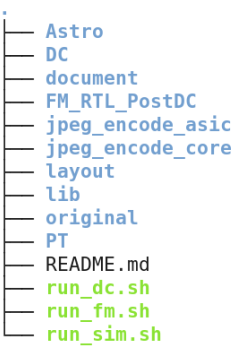
\includegraphics[width =.25\textwidth]{figures/tree.png}
    \caption{工程文件结构}
    \label{tree}
\end{figure}

\subsection{工程的管理}
\subsubsection{版本控制}
编写 \texttt{.gitignore} 文件,忽略不需要版本控制的文件。然后配置好
\texttt{Git} 的用户名和邮箱, 如下所示:
\begin{lstlisting}[style=bashstyle]
    git config --global user.name "Your Name"
    git config --global user.email "Your Email"
\end{lstlisting}

配置\texttt{SSH Key}。将本地仓库与远程仓库关联,
之后执行以下命令,将本地仓库更改推送至远程仓库:
\begin{lstlisting}[style=bashstyle]
    git add .
    git commit -m "Your commit message"
    git push
\end{lstlisting}

\subsubsection{EDA 环境}
在数字集成电路设计课程所提供的虚拟机上执行如下命令,配置 EDA 环境:
\begin{lstlisting}[style=bashstyle]
    source /opt/eda_env.sh
\end{lstlisting}

如果要使用 Astro 进行布局布线,IC5141 和 Calibre 进行后仿真验证,
则需要使用以下命令配置相应环境:
\begin{lstlisting}[style=bashstyle]
    source /opt/eda_env_old.sh
\end{lstlisting}

\newpage
\section{RTL 仿真}
\subsection{仿真环境}
本设计的仿真测试文件为 \texttt{jpeg\_top\_tb.v},仿真测试文件的主要内容如下:

\begin{lstlisting}[style=Verilogstyle,name=jpeg_top_tb]
    `timescale 1ps / 1ps

    module jpeg_top_tb;
    
    reg end_of_file_signal;
    reg [23:0]data_in;
    reg clk;
    reg rst;
    reg enable;
    wire [31:0]JPEG_bitstream;
    wire data_ready;
    wire [4:0]end_of_file_bitstream_count;
    wire eof_data_partial_ready;
    
    // Unit Under Test 
        jpeg_top UUT (
            .end_of_file_signal(end_of_file_signal),
            .data_in(data_in),
            .clk(clk),
            .rst(rst),
            .enable(enable),
            .JPEG_bitstream(JPEG_bitstream),
            .data_ready(data_ready),
            .end_of_file_bitstream_count(end_of_file_bitstream_count),
            .eof_data_partial_ready(eof_data_partial_ready));

    initial
    begin : STIMUL 
        #0
        rst = 1'b1;
        enable = 1'b0;
        end_of_file_signal = 1'b0;
        #10000; 
\end{lstlisting}
\newpage
\begin{lstlisting}[style=Verilogstyle,name=jpeg_top_tb]
        rst = 1'b0;
        enable = 1'b1;
        // data_in holds the red, green, and blue pixel values
        // obtained from the .tif image file
        data_in <= 24'b001101100101001101101110;
    #10000;
    data_in <= 24'b001101110101010001101111;
    #10000;
    /* ... other pixel values */
    data_in <= 24'b001100110011110001010111;
    #10000;
    #130000;
    enable <= 1'b0;
    
    #2000000; 
    
    $finish;
    end // end of stimulus process
        
    always
    begin : CLOCK_clk
        //this process was generated based on formula: 0 0 ns, 1 5 ns -r 10 ns
        //#<time to next event>; // <current time>
        clk = 1'b0;
        #5000; //0
        clk = 1'b1;
        #5000; //5000
    end
    
    always 	@(JPEG_bitstream or data_ready)
    begin : JPEG
            if (data_ready==1'b1) 		
                        $display("%h", JPEG_bitstream);						
    end	
    endmodule
\end{lstlisting}

原设计未提供 Modelsim 的仿真脚本,故需要自行编写仿真脚本,仿真脚本如下:
\newpage
\begin{lstlisting}[style=tclstyle,name=sim.do]
    vlib work
    vmap work work
    vlog -work work ../rtl/*.v jpeg_top_tb.v
    vsim -voptargs=+acc  work.jpeg_top_tb
    add wave  /*
    run 200000000.00 ns
\end{lstlisting}

然后执行 \texttt{vsim -do jpeg\_sim.do} 即可进行仿真。

\subsection{仿真结果}
仿真结果如\autoref{sim}所示,可以看到仿真结果中包含了 JPEG 编码后的比特流。

\begin{figure}[htbp]
    \centering
    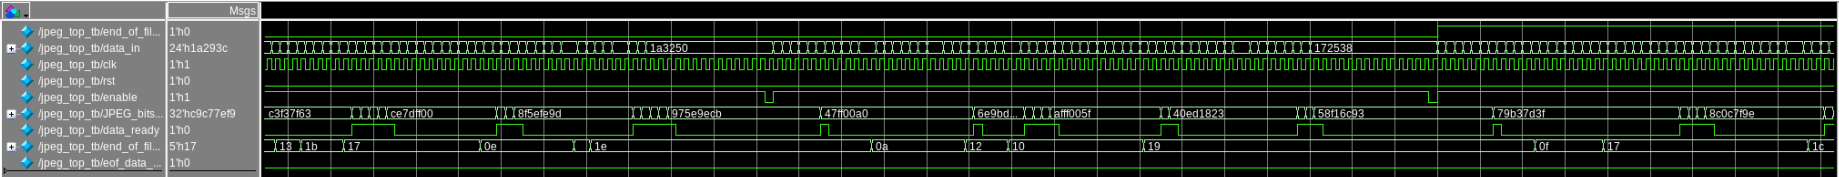
\includegraphics[width =1\textwidth]{figures/sim.png}
    \caption{仿真结果}
    \label{sim}
\end{figure}
该编码器的输入是 24 位数据总线,红色像素、绿色像素和蓝色像素各占 8 位。
信号“data\_in”包含红色像素值([7:0] 位)、绿色像素值([15:8] 位)和蓝色像素值
([23:16] 位)。每个时钟周期应有 24 位数据用于新像素。输入应从图像左上角的 8x8 
块开始,从左上角像素开始,向右,然后向下到第二行,依此类推。在图像的第一个 8x8 
块之后,需要至少延迟 13 个时钟周期才能输入下一个块。然后在此延迟之后,“enable”
信号应在一个时钟周期内变低,然后在下一个时钟周期输入下一个 8x8 块时,“enable”
应变高。图像的第二个 8x8 块应以与第一个块相同的格式输入。第二个 8x8 块将位于
第一个块的右侧。应该从图像的左上角向右移动,直到到达图像的右边缘。然后向下移动
到第二行并继续,直到图像的最后一行。确保在每个块之间插入 13 个或更多时钟周期
的延迟。这是必需的,否则前一个块的计算将尚未完成。

图像数据需要以完整的 8x8 块输入。例如,如果图像是 90 x 90 像素,则需要
将像素数据扩展为 96 x 96 像素。这通常是通过将边缘像素值重复到每行或每列的额外像素上来实现的。

输入最后一个 8x8 像素数据块时,在块开头置位信号“end\_of\_file\_signal”。这让
其知道没有更多块需要输入,剩余的位将被输出,即使它们没有填满完整的 32 位。
如果最后的 JPEG 位不是完整的 32 位,则信号“eof\_data\_partial\_ready”将在
一个时钟周期内保持高电平,并且信号“JPEG\_bitstream”中的位将在一个时钟周期
内保持有效。信号“end\_of\_file\_bitstream\_count”中的值表示在图像文件末尾信
号“JPEG\_bitstream”中有多少位有效。

输出是信号“JPEG\_bitstream”,它是一个 32 位宽度的总线。位是按大端对齐的
,因此占据位置 31-24 的位是输出的前 8 位,后面是 23-16,依此类推。当信
号“data\_ready”变为高电平时,信号“JPEG\_bitstream”中的数据有效。位流数据
将在第一个块输入后不久输出,并在像素数据输入到核心时继续输出。

原始项目中包含一个示例测试文件“jpeg\_top\_tb.v”。这给出了运行核心所需
时间的示例。来自图像文件“ja.tif”的数据用作测试台中的像素数据输入。核心
的输出位于文件“ja\_bits\_out.v”中。这些位用于创建 jpeg 图像“ja.jpg”。需
要单独创建文件的标头。JPEG 编码器核心不会创建 jpeg 标头文件。此外,
需要在 JPEG 位后添加“FFD9”(扫描结束标记)才能完成 JPEG 文件。此核心仅
输出由 Huffman 码创建的 JPEG 位。可以使用 MATLAB 程序从单独的标头和
从此 JPEG 编码器创建的 jpeg 位创建“ja.jpg”图像。

\newpage

\section{综合与形式验证}

\subsection{原设计 RTL 代码的修改}
为了进行后续自动布局布线步骤,在原设计顶层模块 \texttt{jpeg\_top} 上添加了 PAD ,
主要代码如下:
\begin{lstlisting}[style=Verilogstyle,name=jpeg_asic]
    module jpeg_asic(
        PAD_clk_i, 
        PAD_rst_i, 
        PAD_eof_signal_i, 
        PAD_enable_i, 
        PAD_dat_i, 
        PAD_jpeg_bitstr_o, 
        PAD_dat_rdy_o, 
        PAD_eof_bitstr_cnt_o, 
        PAD_eof_dat_partial_rdy_o
        );
    
    input PAD_clk_i;
    input PAD_rst_i;
    input PAD_eof_signal_i;
    input PAD_enable_i;
    input [23:0] PAD_dat_i;
    output [31:0] PAD_jpeg_bitstr_o;
    output PAD_dat_rdy_o;
    output [4:0] PAD_eof_bitstr_cnt_o;
    output PAD_eof_dat_partial_rdy_o;
    
    wire           clk;
    wire           rst;
    wire           end_of_file_signal;
    wire           enable;
    wire   [23:0]  data_in;
    wire  [31:0]  JPEG_bitstream;
    wire          data_ready;
    wire  [4:0] end_of_file_bitstream_count;
    wire          eof_data_partial_ready;
\end{lstlisting}
\newpage
\begin{lstlisting}[style=Verilogstyle,name=jpeg_asic]
    //PAD
    //in
    PLBI8F  U_clk_i      (.D( clk ), .P( PAD_clk_i ), .A( 1'b0 ), .CONOF( 1'b1 ), .NEN( 1'b0 ), .PD( 1'b0 ), .PEN( 1'b0 ), .PU( 1'b1 ), .SONOF( 1'b0 ));
    PLBI8F  U_rst_i      (.D( rst ), .P( PAD_rst_i ), .A( 1'b0 ), .CONOF( 1'b1 ), .NEN( 1'b0 ), .PD( 1'b0 ), .PEN( 1'b0 ), .PU( 1'b1 ), .SONOF( 1'b0 ));
    PLBI8F  U_eof_signal_i      (.D( end_of_file_signal ), .P( PAD_eof_signal_i ), .A( 1'b0 ), .CONOF( 1'b1 ), .NEN( 1'b0 ), .PD( 1'b0 ), .PEN( 1'b0 ), .PU( 1'b1 ), .SONOF( 1'b0 ));
    /* ... other input ports */

    //out
    PLBI8F	U_dat_o_0	(.D(  ), .P( PAD_jpeg_bitstr_o[0] ), .A( JPEG_bitstream[0] ), .CONOF( 1'b0 ), .NEN( 1'b1 ), .PD( 1'b0 ), .PEN( 1'b1 ), .PU( 1'b1 ), .SONOF( 1'b0 )); 
    PLBI8F	U_dat_o_1	(.D(  ), .P( PAD_jpeg_bitstr_o[1] ), .A( JPEG_bitstream[1] ), .CONOF( 1'b0 ), .NEN( 1'b1 ), .PD( 1'b0 ), .PEN( 1'b1 ), .PU( 1'b1 ), .SONOF( 1'b0 )); 
    /* ... other output ports */
    
    jpeg_top jpeg_top_inst(
        .clk(clk), 
        .rst(rst), 
        .end_of_file_signal(end_of_file_signal), 
        .enable(enable), 
        .data_in(data_in), 
        .JPEG_bitstream(JPEG_bitstream),
        .data_ready(data_ready), 
        .end_of_file_bitstream_count(end_of_file_bitstream_count), 
        .eof_data_partial_ready(eof_data_partial_ready)
        );
    
    endmodule
\end{lstlisting}

\subsection{DC 综合}
综合就是把行为级的RTL代码在工艺、面积、时序等约束下转换成对应的门级网表,
是使用软件来设计硬件,然后将门级电路实现与优化的工作留给综合工具的一种设计方法。

DC综合分为三阶段:转换、优化、映射。主要流程为读入设计、设置约束、执行综合、
查看报告、保存结果。综合的目标是生成一个满足约束条件的电路,同时尽可能满足
电路的面积、功耗和时延。

\subsubsection{环境配置}
在综合之前,需要修改 \texttt{.synopsys\_dc.setup} 文件,如下所示:

\begin{lstlisting}[style=tclstyle,name=.synopsys_dc.setup]
    set topDir              "../jpeg_encode_asic/rtl"
\end{lstlisting}

其他内容与 aes\_asic 的配置相同,完整内容见仓库 \texttt{DC/.synopsys\_dc.setup} 文件。

\subsubsection{读入设计}
在 aes\_asic 所提供 \texttt{DC/scripts} 目录下的 \texttt{read\_rtl.tcl} 文件
基础上修改,如下所示:

\begin{lstlisting}[style=tclstyle,name=read_rtl.tcl]
    set TOP_MODULE  jpeg_asic
\end{lstlisting}

完整内容见仓库 \texttt{DC/scripts/read\_rtl.tcl} 文件。然后在 \texttt{DC} 目录下执行
aes\_asic 所提供 shell 脚本 \texttt{run\_dc\_read\_rtl.sh} 即可读入设计。
\begin{figure}[htbp]
    \centering
    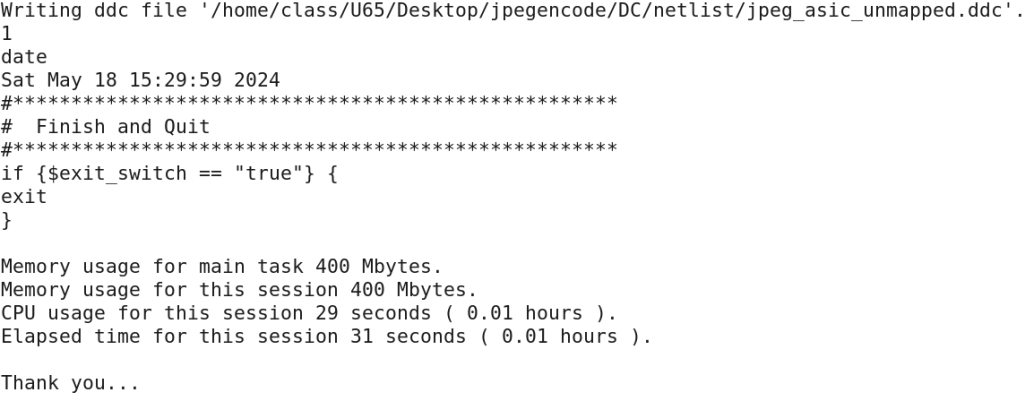
\includegraphics[width =0.9\textwidth]{figures/dc_read_rtl.png}
    \caption{读入设计脚本执行结果}
    \label{dc_read_rtl}
\end{figure}

\subsubsection{设置约束}
在 aes\_asic 所提供 \texttt{DC/scripts} 目录下的 \texttt{constraint\_compile.tcl} 文件
基础上修改,如下所示:

\begin{lstlisting}[style=tclstyle,name=constraint_compile.tcl]
    set TOP_MODULE          jpeg_asic
    set Rst_list            [list PAD_rst_i]
\end{lstlisting}

\begin{lstlisting}[style=tclstyle,name=constraint_compile.tcl]
    set Clk_list            [list PAD_clk_i]
    
    # other unchanged content
    
    create_clock -name wb_clk -period $SYS_CLK_PERIOD -waveform [list 0 [expr $SYS_CLK_PERIOD /2]]  [get_ports PAD_clk_i]
    
    # other unchanged content
    
    set_ideal_network [get_pins "U_clk_i/D"]
    
    # other unchanged content
    
    set wb_in_ports [remove_from_collection [all_inputs]  [get_ports [list PAD_clk_i PAD_rst_i]]]
    set wb_out_ports [get_ports [list PAD_jpeg_bitstr_o PAD_dat_rdy_o PAD_eof_bitstr_cnt_o PAD_eof_dat_partial_rdy_o]]

    set_case_analysis 0 [get_pins "U_rst_i/D"]
\end{lstlisting}

另外,根据设计要求:
\begin{itemize}
    \item 时钟频率为 50\unit{\MHz},\texttt{uncertainy} 为 0.1\unit{\ns}
    \item 驱动 \texttt{cell} 设为 \texttt{INVHD2X} ,负载设为 \texttt{3 x INVHD4X}
    \item \texttt{input\_delay} 和 \texttt{output\_delay} 按 50\% 时钟预算
\end{itemize}
脚本修改内容如下:
\begin{lstlisting}[style=tclstyle,name=constraint_compile_1.tcl]
    set SYS_CLK_PERIOD 20.0
    set_clock_uncertainty   0.1     [all_clocks]
    
    set MAX_LOAD [load_of smic18_ss/INVHD4X/A]
    set_driving_cell -lib_cell INVHD2X [remove_from_collection [all_inputs] \
         [get_ports [list PAD_clk_i PAD_rst_i]]]
    set_load [expr $MAX_LOAD*3] [all_outputs]

    set_input_delay -max 10 -clock wb_clk $wb_in_ports
    set_input_delay -min 0.1 -clock wb_clk $wb_in_ports
    set_output_delay -max 10 -clock wb_clk $wb_out_ports
    set_output_delay -min -1 -clock wb_clk $wb_out_ports
\end{lstlisting}

完整内容见仓库 \texttt{DC/scripts/constraint\_compile.tcl} 文件。然后在 \texttt{DC} 目录下执行
aes\_asic 所提供 shell 脚本 \texttt{run\_dc\_constraint\_compile.sh} 即可设置约束并完成综合。
\begin{figure}[htbp]
    \centering
    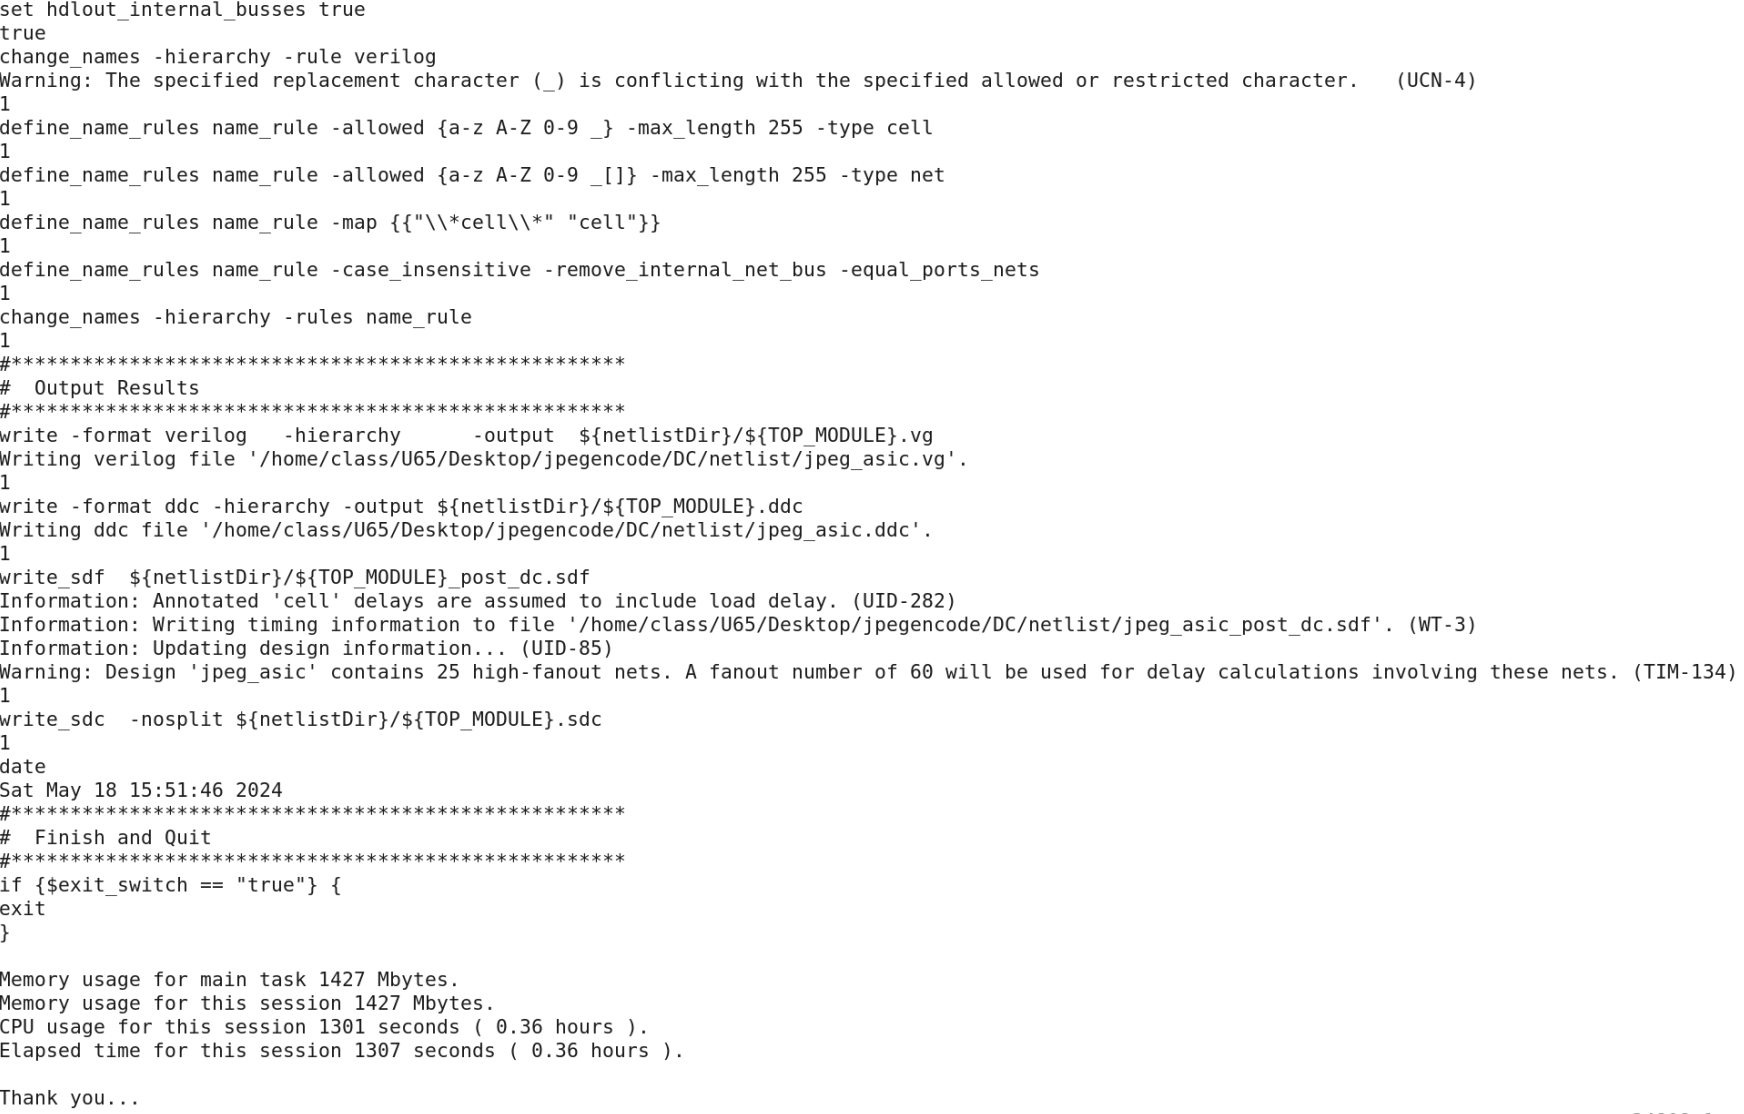
\includegraphics[width =.9\textwidth]{figures/dc_constraint_compile.png}
    \caption{设置约束及综合脚本执行结果}
    \label{dc_constraint_compile}
\end{figure}

\subsubsection{查看报告}
综合完成后,可以查看综合报告,报告中包含了综合后的面积、时序等信息。

采用 SMIC18 工艺库综合后,整个设计的面积为 9559257,如\autoref{dc_area}所示。
\begin{figure}[htbp]
    \centering
    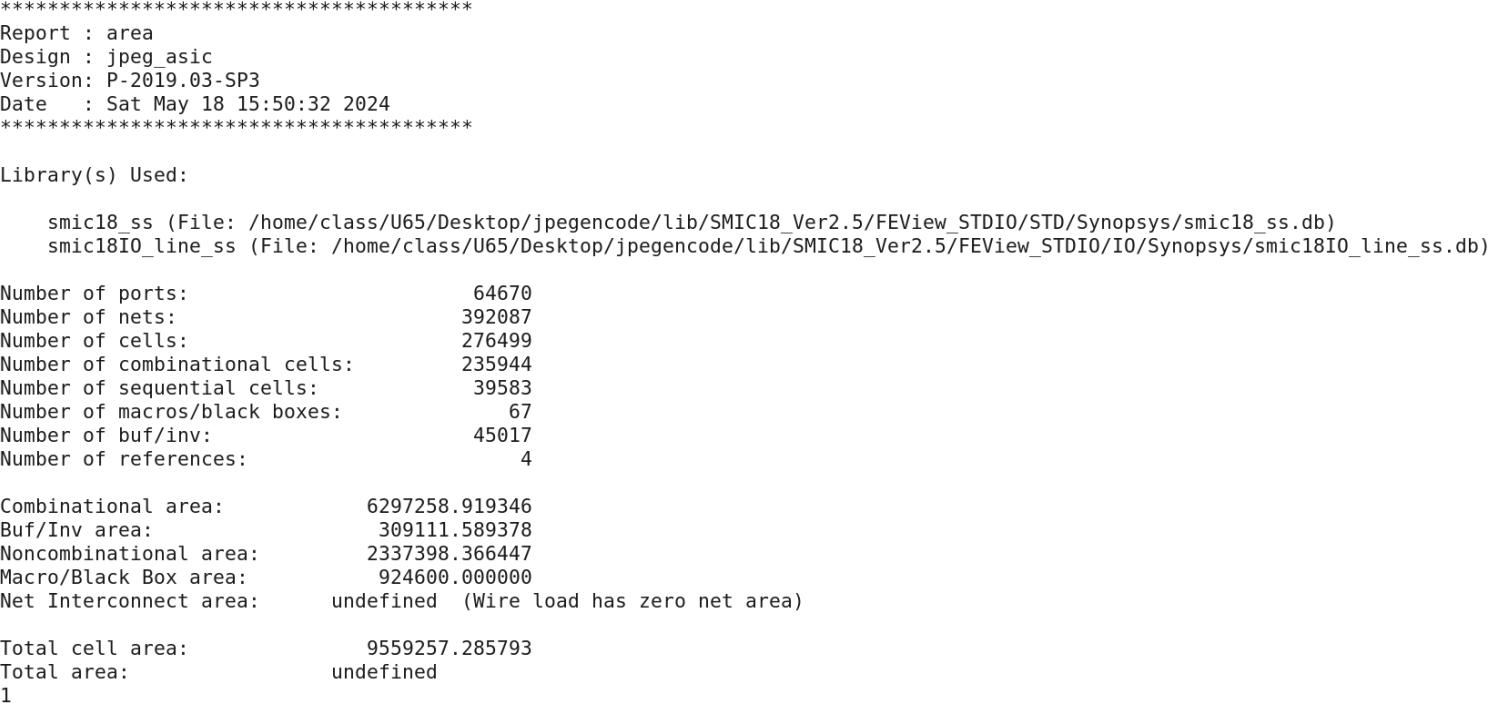
\includegraphics[width =.9\textwidth]{figures/dc_area.png}
    \caption{综合面积报告}
    \label{dc_area}
\end{figure}
\newpage

当前时序约束下,时序报告如\autoref{dc_timing}所示。

\begin{figure}[htbp]
    \centering
    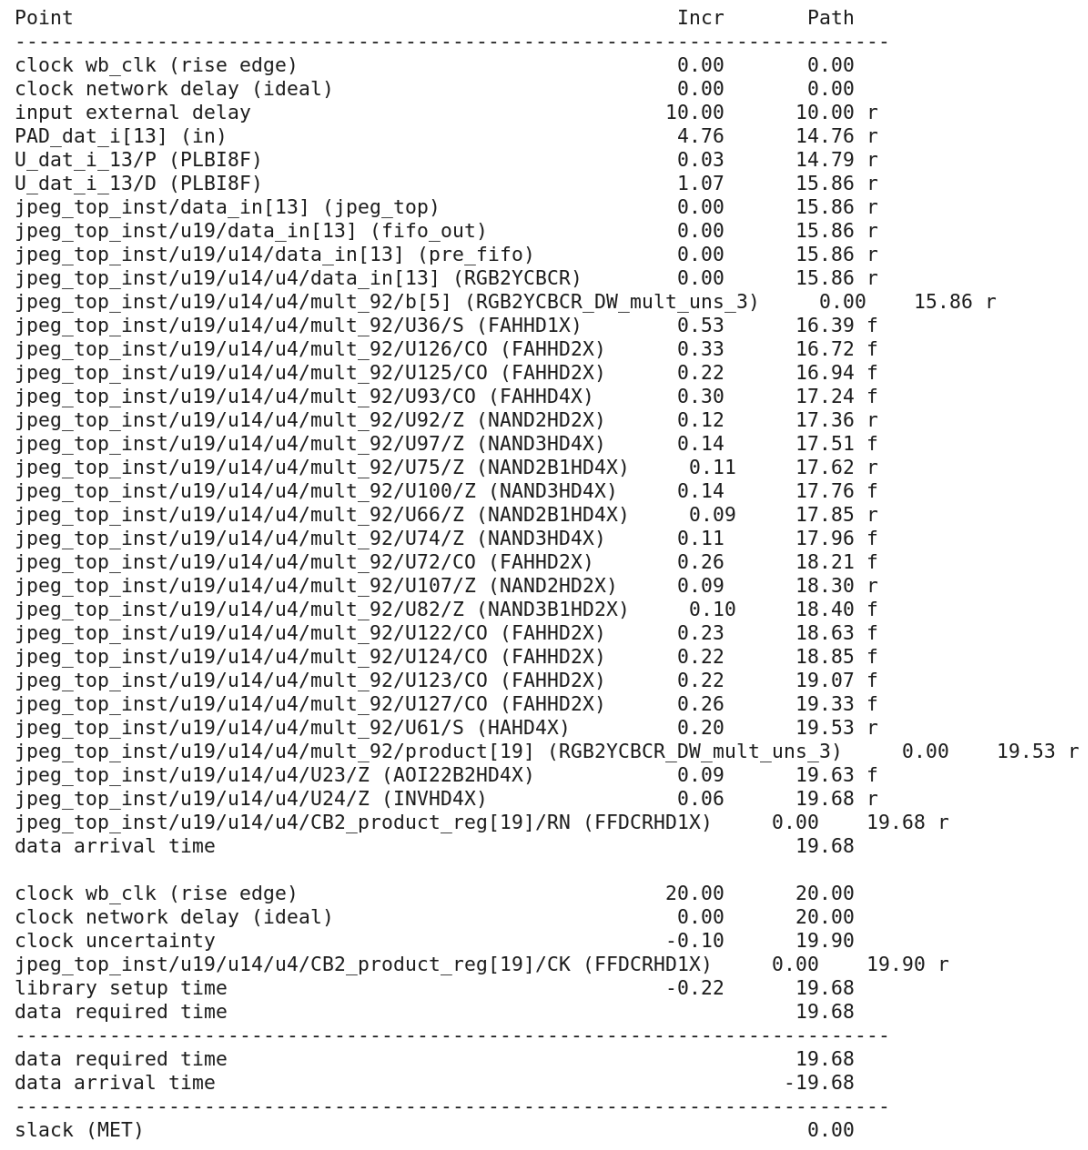
\includegraphics[width =.6\textwidth]{figures/dc_timing.png}
    \caption{综合时序报告}
    \label{dc_timing}
\end{figure}
由图可知, data required time 为 19.68\unit{\ns}, data arrival time 为 -19.68\unit{\ns},slack 为 0。
满足时序约束。

功耗报告如\autoref{dc_power}所示。可知功耗约为 170.2820\unit{\mW}。
\begin{figure}[htbp]
    \centering
    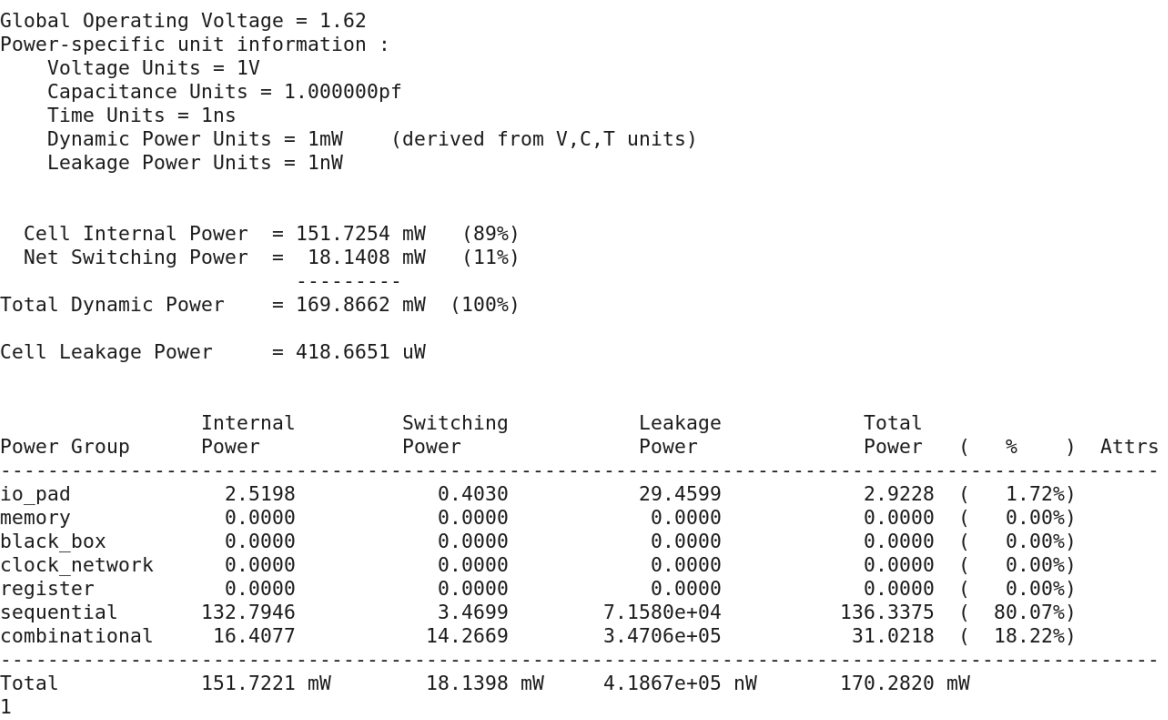
\includegraphics[width =.6\textwidth]{figures/dc_power.png}
    \caption{综合功耗报告}
    \label{dc_power}
\end{figure}

\subsection{形式验证}
在综合、适配过程后,要确保电路功能不变。后仿真是一种方法,但是后仿真时间精度高,
仿真时间长。当设计规模很大时,仿真时间会很长。可以进行分别处理时序分析采用 STA,
功能验证采用形式验证。形式验证是一种数学方法,通过数学方法证明电路功能正确。
与 RTL 仿真相比,RTL 仿真证明 RTL 功能正确,时间较短,需要保证一定的测试覆盖率。
形式验证证明 RTL 与 Gate 代码等价,则说明 Gate 功能也正确。STA 证
明 Gate 代码满足时序要求,则证明 Gate 级代码功能、时序均满足。
形式验证流程图如\autoref{fm_flow}所示。

\begin{figure}[htbp]
    \centering
    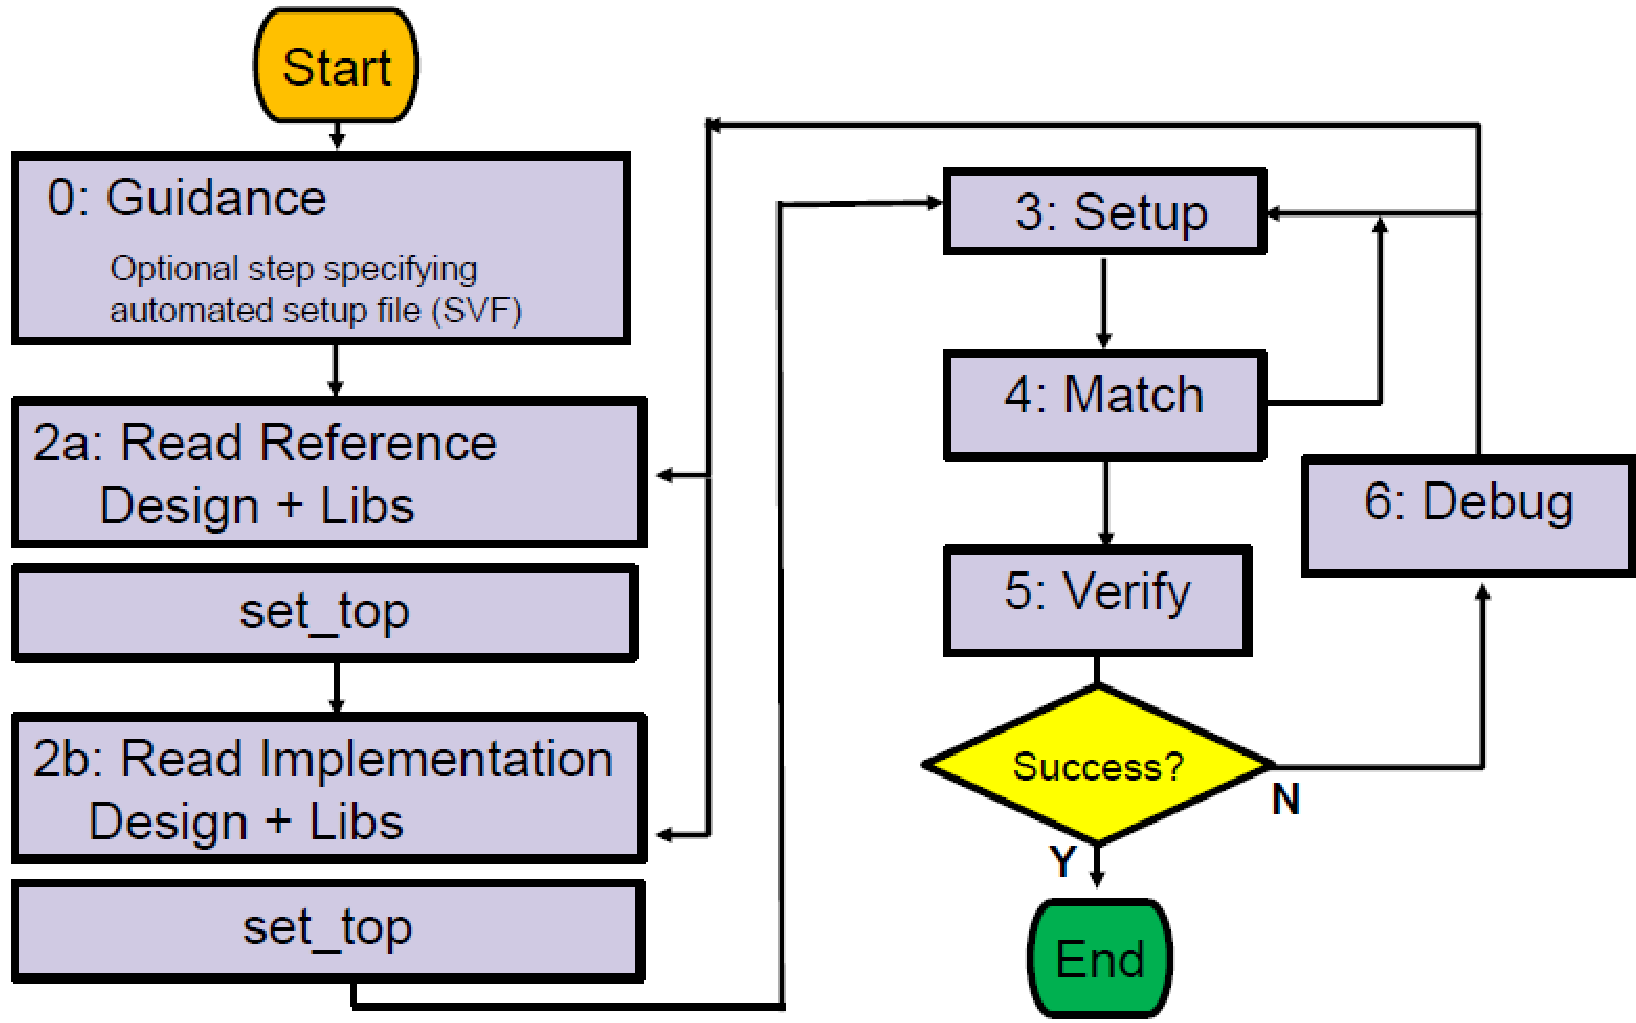
\includegraphics[width =.45\textwidth]{figures/fm_flow.png}
    \caption{形式验证流程图}
    \label{fm_flow}
\end{figure}

\subsubsection{形式验证步骤}
在形式验证之前,据 aes\_asic 所提供的环境稍作修改,将 \texttt{FM\_RTL\_PostDC/netlist}
链接至 DC 综合后生成结果的文件夹。 执行如下命令:
\begin{lstlisting}[style=bashstyle]
    ln -snf ../DC/netlist/ netlist
\end{lstlisting}

将 \texttt{FM\_RTL\_PostDC/netlist} 链接至 本设计 RTL 代码所在文件夹。 
执行如下命令:
\begin{lstlisting}[style=bashstyle]
    ln -snf ../jpeg_encode_asic/rtl rtl
\end{lstlisting}

在 aes\_asic 所提供 \texttt{FM\_RTL\_PostDC} 目录下的 \texttt{.fms} 文件
基础上修改,并重命名为 \texttt{jpeg\_encode\_asic.fms},完整内容如下所示:
\begin{lstlisting}[style=tclstyle,name=jpeg_encode_asic.fms]
    date
    set TOP_MODULE jpeg_asic
    set     search_path     "$search_path  $topDir "
    set     synopsys_auto_setup     true
    set_svf ${svfDir}/${TOP_MODULE}.svf
    read_db "lib/SMIC18_Ver2.5/FEView_STDIO/STD/Synopsys/smic18_tt.db lib/SMIC18_Ver2.5/FEView_STDIO/IO/Synopsys/smic18IO_line_tt.db"
\end{lstlisting}
\begin{lstlisting}[style=tclstyle,name=jpeg_encode_asic.fms]
    read_verilog -r [sh ls $topDir/*.v]
    set_top ${TOP_MODULE}
    read_verilog -i ${TOP_MODULE}.vg
    set_top ${TOP_MODULE}
\end{lstlisting}

然后对 \texttt{run\_fm.scr} 修改,如下所示:

\begin{lstlisting}[style=bashstyle,name=run_fm.scr]
    #!/bin/sh
    mkdir -p logs
    fm_shell -f jpeg_encode_asic.fms | tee -i logs/jpeg_encode_asic.log
\end{lstlisting}

在 \texttt{FM\_RTL\_PostDC} 目录下执行 aes\_asic 所提供 shell 
脚本 \texttt{run\_fm.scr} 即可进行形式验证。形式验证结果如\autoref{fm}所示。

\begin{figure}[htbp]
    \centering
    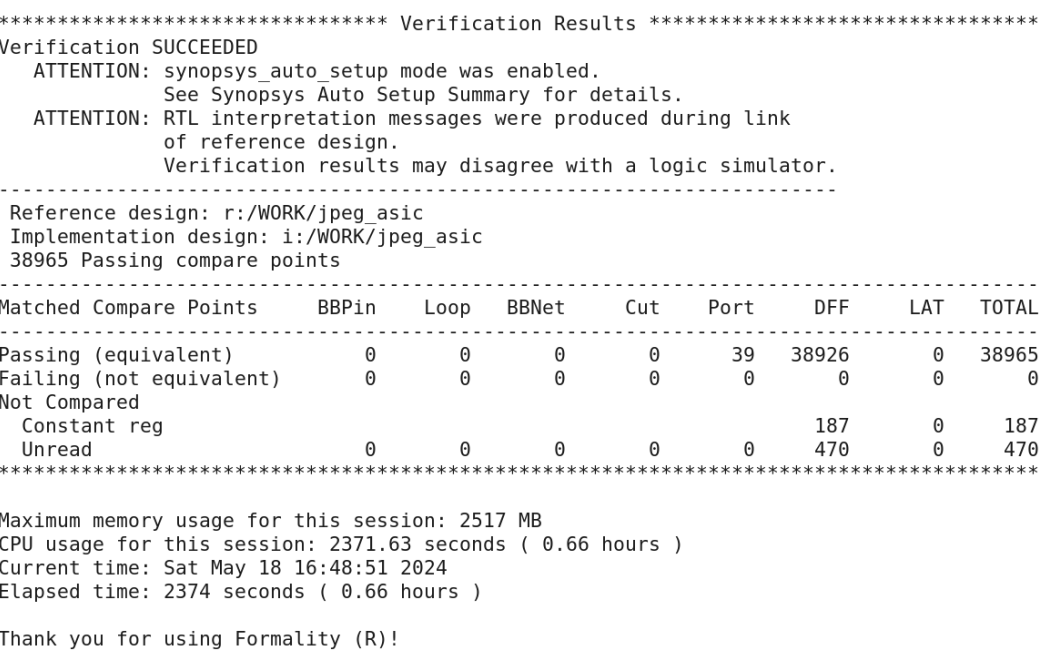
\includegraphics[width =.8\textwidth]{figures/fm.png}
    \caption{形式验证结果}
    \label{fm}
\end{figure}
\newpage
\section{自动布局布线}
\subsection{设计输入}
执行 \texttt{prep\_fend\_data.sh} 脚本,将门级网表、设计约束、
工艺库等导入到 Astro 目录下并对约束进行处理使 Astro 可以读入。
脚本内容如下:
\begin{lstlisting}[style=bashstyle, name=prep_fend_data.sh]
    #!/bin/bash

    TOP_MODULE=jpeg_asic
    cp ../DC/netlist/${TOP_MODULE}.vg ./data_fend
    cp ../DC/netlist/${TOP_MODULE}.sdc ./data_fend
    cp ../DC/netlist/${TOP_MODULE}.ddc ./data_fend
    
    (cd data_fend; ./prep_sdc.sh ${TOP_MODULE}.sdc)
\end{lstlisting}
    
根据 aes\_asic 提供的脚本,修改 \texttt{Astro/soc\_scripts/1.0\_design\_setup.cmd}
文件,主要内容如下所示:
\begin{lstlisting}[style=tclstyle,name=1.0_design_setup.cmd]
    ;# Scheme
    menuReload "astro_data_prep"
    auVerilogToCell
    formDefault "Verilog To Cell"
    setFormField "Verilog To Cell" "Library Name" "design_lib_jpeg_asic"
    setFormField "Verilog To Cell" "Verilog File Name" "./data_fend/jpeg_asic.vg"
    setFormField "Verilog To Cell" "Output Cell Name" "jpeg_asic"
    setFormField "Verilog To Cell" "Top Module Name" "jpeg_asic"
    setFormField "Verilog To Cell" "Tech File Name" "../lib//SMIC18_Ver2.5/BEView_STDIO/TECH/smic18_apollo_m6.tf"
    setFormField "Verilog To Cell" "Net Name for 1'b0" "GND"
    setFormField "Verilog To Cell" "Open Library and Cell When Done" "1"
    setFormField "Verilog To Cell" "Initialize Hierarchy Preservation" "1"
    formButton "Verilog To Cell" "globalNetOptions"
    setFormField "Verilog To Cell" "Net Name" "VDD"
    setFormField "Verilog To Cell" "Port Pattern" "VDD"
    formButton "Verilog To Cell" "apply"
    setFormField "Verilog To Cell" "Net Name" "GND"
    setFormField "Verilog To Cell" "Port Pattern" "GND"

    ;# other unchanged content
\end{lstlisting}

\subsection{布局规划}
\subsubsection{电源引脚规划}
首先,根据 aes\_asic 的 \texttt{.tdf} 文件,修改 \texttt{.tdf} 文件。
要规划电源引脚个数,有两种电源引脚:core 供电 PAD (PLVDDC/PLVSSC, 1.8\unit{\V})、
IO 供电 PAD (PLVDDH/
PLVSSH, 3.3\unit{\V})。根据功耗、电流信息计算,但最好是大于
此计算值,一般还会考虑对称性,供电均匀。

本设计中,根据综合报告,如\autoref{dc_power}所示,
功耗约为 170.2820 \unit{\mW}。考虑较差情况,电压取值 1.6\unit{\V}。PAD 与 
core ring 连接金属为 35\unit{\um}时,
最大电流应该按 35\unit{\mA} 计算。则需要的 core 供电 PAD 数:
\begin{equation}
    \dfrac{\dfrac{170.2820}{1.6}}{35} \approx 3.04 
\end{equation}
因此安排 4 对,4 面各 1 对。

PAD 供电电源数量估算考虑最坏情况,即所有的输出 PAD 与双向 PAD 同时输出。需要的 IO 供电 PAD 数:
\begin{equation}
    \dfrac{39 \times 8}{51} \approx 6.12
\end{equation}
安排 8 对,4 面各 2 对。

\texttt{.tdf} 文件主要内容如下:
\begin{lstlisting}[style=tdfstyle,name=jpeg_asic.tdf]
    ;TDF file for jpeg_asic
    ;Chip Directions
    ;;;;;;;;;;;;;;;;;;;;;;;;;;;;;;;;;;;;;;;;
    ;		(Top)		       ;
    ;(Left)				(Right);
    ;		(Bottom)	       ;
    ;;;;;;;;;;;;;;;;;;;;;;;;;;;;;;;;;;;;;;;;
    define _cell (geGetEditCell)

    ;pad record section
    tdfPurgePadConstr
    tdfSetMinIODistance 0 0 0 0

    ;use insertPad or dbCreateCellInst for PLVDD* and PLVSS*
    dbCreateNet _cell "VDDH"
    dbCreateNet _cell "VSSH"
\end{lstlisting}

\newpage
\begin{lstlisting}[style=tdfstyle,name=jpeg_asic.tdf]
    insertPad "VDDH" "PLVDDH" "pad_L_VDDH1" "VDDH"
    insertPad "VDDH" "PLVDDH" "pad_L_VDDH2" "VDDH"
    insertPad "VDDH" "PLVDDH" "pad_L_VDDH3" "VDDH"
    insertPad "VDDH" "PLVDDH" "pad_L_VDDH4" "VDDH"
    insertPad "VDDH" "PLVDDH" "pad_L_VDDH5" "VDDH"
    insertPad "VDDH" "PLVDDH" "pad_L_VDDH6" "VDDH"
    insertPad "VDDH" "PLVDDH" "pad_L_VDDH7" "VDDH"
    insertPad "VDDH" "PLVDDH" "pad_L_VDDH8" "VDDH"

    insertPad "VSSH" "PLVSSH" "pad_L_VSSH1" "VSSH"
    insertPad "VSSH" "PLVSSH" "pad_L_VSSH2" "VSSH"
    insertPad "VSSH" "PLVSSH" "pad_L_VSSH3" "VSSH"
    insertPad "VSSH" "PLVSSH" "pad_L_VSSH4" "VSSH"
    insertPad "VSSH" "PLVSSH" "pad_L_VSSH5" "VSSH"
    insertPad "VSSH" "PLVSSH" "pad_L_VSSH6" "VSSH"
    insertPad "VSSH" "PLVSSH" "pad_L_VSSH7" "VSSH"
    insertPad "VSSH" "PLVSSH" "pad_L_VSSH8" "VSSH"

    insertPad "VDD" "PLVDDC" "pad_L_VDDC1" "VDD"
    insertPad "VDD" "PLVDDC" "pad_L_VDDC2" "VDD"
    insertPad "VDD" "PLVDDC" "pad_L_VDDC3" "VDD"
    insertPad "VDD" "PLVDDC" "pad_L_VDDC4" "VDD"

    insertPad "GND" "PLVSSC" "pad_L_VSSC1" "GND"
    insertPad "GND" "PLVSSC" "pad_L_VSSC2" "GND"
    insertPad "GND" "PLVSSC" "pad_L_VSSC3" "GND"
    insertPad "GND" "PLVSSC" "pad_L_VSSC4" "GND"

    insertPad "GND" "PLCORNER" "corner_ll" "GND"
    insertPad "GND" "PLCORNER" "corner_lr" "GND"
    insertPad "GND" "PLCORNER" "corner_ul" "GND"
    insertPad "GND" "PLCORNER" "corner_ur" "GND"

    pad	"corner_ll"	"bottom" 	
    pad	"corner_ul"	"left"	 
    pad	"corner_lr"	"right"	 	
    pad	"corner_ur"	"top"	 
\end{lstlisting}
\newpage
\begin{lstlisting}[style=tdfstyle,name=jpeg_asic.tdf]
    ; Bottom ( --> 23 pads )	 
    pad "U_dat_i_0" 	"bottom" 	1
    pad "U_dat_i_1" 	"bottom" 	2
    pad "U_dat_i_2" 	"bottom" 	3
    pad "U_dat_i_3" 	"bottom" 	4
    pad "U_dat_i_4" 	"bottom" 	5
    pad "pad_L_VSSH1"	"bottom" 	6
    pad "pad_L_VDDH1" 	"bottom" 	7
    pad "U_dat_i_5" 	"bottom" 	8
    ; ... other pads

    ;Right ( --> 23 pads)
    pad "U_dat_i_17" 	"right"	    1
    pad "U_dat_i_18" 	"right"		2
    pad "U_dat_i_19" 	"right"		3
    pad "U_dat_i_20" 	"right"		4
    pad "U_dat_i_21" 	"right"		5
    pad "pad_L_VSSH3"	"right" 	6
    pad "pad_L_VDDH3" 	"right" 	7
    pad "U_dat_i_22" 	"right"		8
    pad "U_dat_i_23" 	"right" 	9
    pad "U_dat_o_0" 	"right"		10
    pad "U_dat_o_1" 	"right"	    11
    pad "pad_L_VDDC2"	"right"		12
    pad "pad_L_VSSC2"	"right" 	13
    pad "U_dat_o_2" 	"right"		14	
    ; ... other pads

    ; Top ( --> 23 pads )
    pad "U_dat_o_10" 	"top"		1
    pad "U_dat_o_11" 	"top"		2
    ; ... other pads

    ; Left( --> 22 pads)
    pad "U_dat_o_27" 	            "left"		1
    ; ... other pads
    ;;Finished
\end{lstlisting}
完整内容见仓库 \texttt{Astro/jpeg\_asic.tdf} 文件。

\subsubsection{芯片大小估算}
根据公式计算芯片面积:
\begin{equation}
    (23 \times 74 + 184 \times 2)- 80 \times 2 - 184\times 2 = 1542
\end{equation}

考虑一定余量,根据该公式分别设置芯片的长宽为 2500,但是在布局规划过程中,
Astro 报错,提示芯片面积不够,如下图所示。
\begin{figure}[htbp]
    \centering
    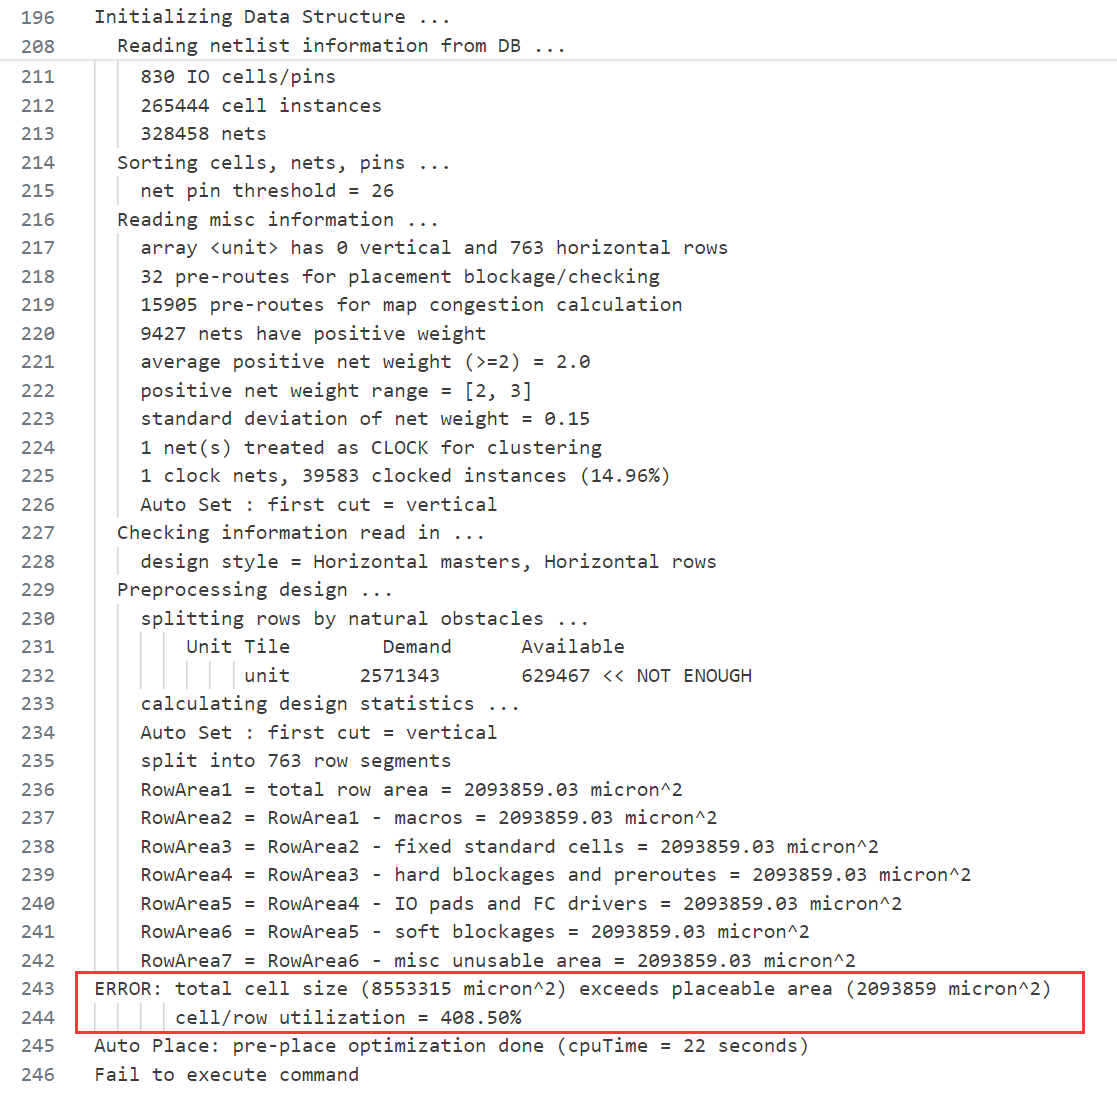
\includegraphics[width =.8\textwidth]{figures/astro_floorplan_err.png}
    \caption{Astro 报错}
    \label{astro_error}
\end{figure}

该错误是 core limited, 根据报错给出的大小,进行计算。
\begin{equation}
    \sqrt{8553315} \approx 2925
\end{equation}

因此设置芯片的长宽为 5000,重新进行布局规划。
修改 \texttt{Astro/soc\_scripts} 目录下的 \texttt{2.0\_floorplan\_before\_place\_macro.cmd} 
文件,主要内容如下所示:
\begin{lstlisting}[style=tclstyle,name=2.0_floorplan_before_place_macro]
    ;# Scheme
    geOpenLib
    formDefault "Open Library"
\end{lstlisting}

\begin{lstlisting}[style=tclstyle,name=2.0_floorplan_before_place_macro]
    setFormField "Open Library" "Library Name" "design_lib_jpeg_asic"
    formOK "Open Library"
    geOpenCell
    formDefault "Open Cell"
    setFormField "Open Cell" "Cell Name" "10_design_setup"
    formOK "Open Cell"
    
    axgLoadTDF
    formDefault "Load TDF File"
    setFormField "Load TDF File" "TDF File Name" "jpeg_asic.tdf"
    setFormField "Load TDF File" "Cell Name" "10_design_setup"
    formOK "Load TDF File"
    
    axgPlanner
    formDefault "Floor Planning"
    setFormField "Floor Planning" "Control Parameter" "width & height"
    setFormField "Floor Planning" "Row/Core Ratio" "0.75"
    
    setFormField "Floor Planning" "Core Width" "5000"
    setFormField "Floor Planning" "Core Height" "5000"
    setFormField "Floor Planning" "Core To Left" "80"
    setFormField "Floor Planning" "Core To Bottom" "80"
    setFormField "Floor Planning" "Core To Right" "80"
    setFormField "Floor Planning" "Core To Top" "80"
    setFormField "Floor Planning" "Double Back" "1"
    setFormField "Floor Planning" "Start from first row" "1"
    setFormField "Floor Planning" "Flip first row" "1"
    formOK "Floor Planning"

    ;# other unchanged content
\end{lstlisting}
\subsubsection{添加 PAD filler 、电源环、电源条等}
然后在 PAD 中间填充 PAD filler, Pad 之间的缝隙需要填充,PAD 之间无连线,
电源、地在相同位置,用 Filler 连接起来,形成 Pad rings 环。
再将电源 PAD 与 core ring 连接起来。完成后结果如\autoref{astro_floorplan}所示。

修改所提供的 \texttt{createstrap.cmd} 文件,如下所示:
\newpage
\begin{lstlisting}[style=tclstyle,name=createstrap.cmd]
    axgCreateStraps
    setFormField "Create Straps" "Direction" "Vertical"
    setFormField "Create Straps" "Start X" "800"
    setFormField "Create Straps" "Net Name(s)" "VDD,VDD,GND,GND"
    setFormField "Create Straps" "Width" "18"
    setFormField "Create Straps" "Layer" "66"
    setFormField "Create Straps" "Extend for Multiple Connections" "1"
    setFormField "Create Straps" "For Gap <" "2"
    formApply "Create Straps"
    setFormField "Create Straps" "Start X" "1500"
    formApply "Create Straps"
    setFormField "Create Straps" "Start X" "2200"
    formApply "Create Straps"
    setFormField "Create Straps" "Start X" "2900"
    formApply "Create Straps"
    setFormField "Create Straps" "Start X" "3600"
    formApply "Create Straps"
    setFormField "Create Straps" "Start X" "4300"
    formOK "Create Straps"
\end{lstlisting}

在适当的位置添加电源条,方便个cell电压均匀,添加了电源条的版图如\autoref{astro_floorplan_add_strap}所示。
\begin{figure}[htbp]
    \centering
    \begin{minipage}{0.45\textwidth}
        \centering
        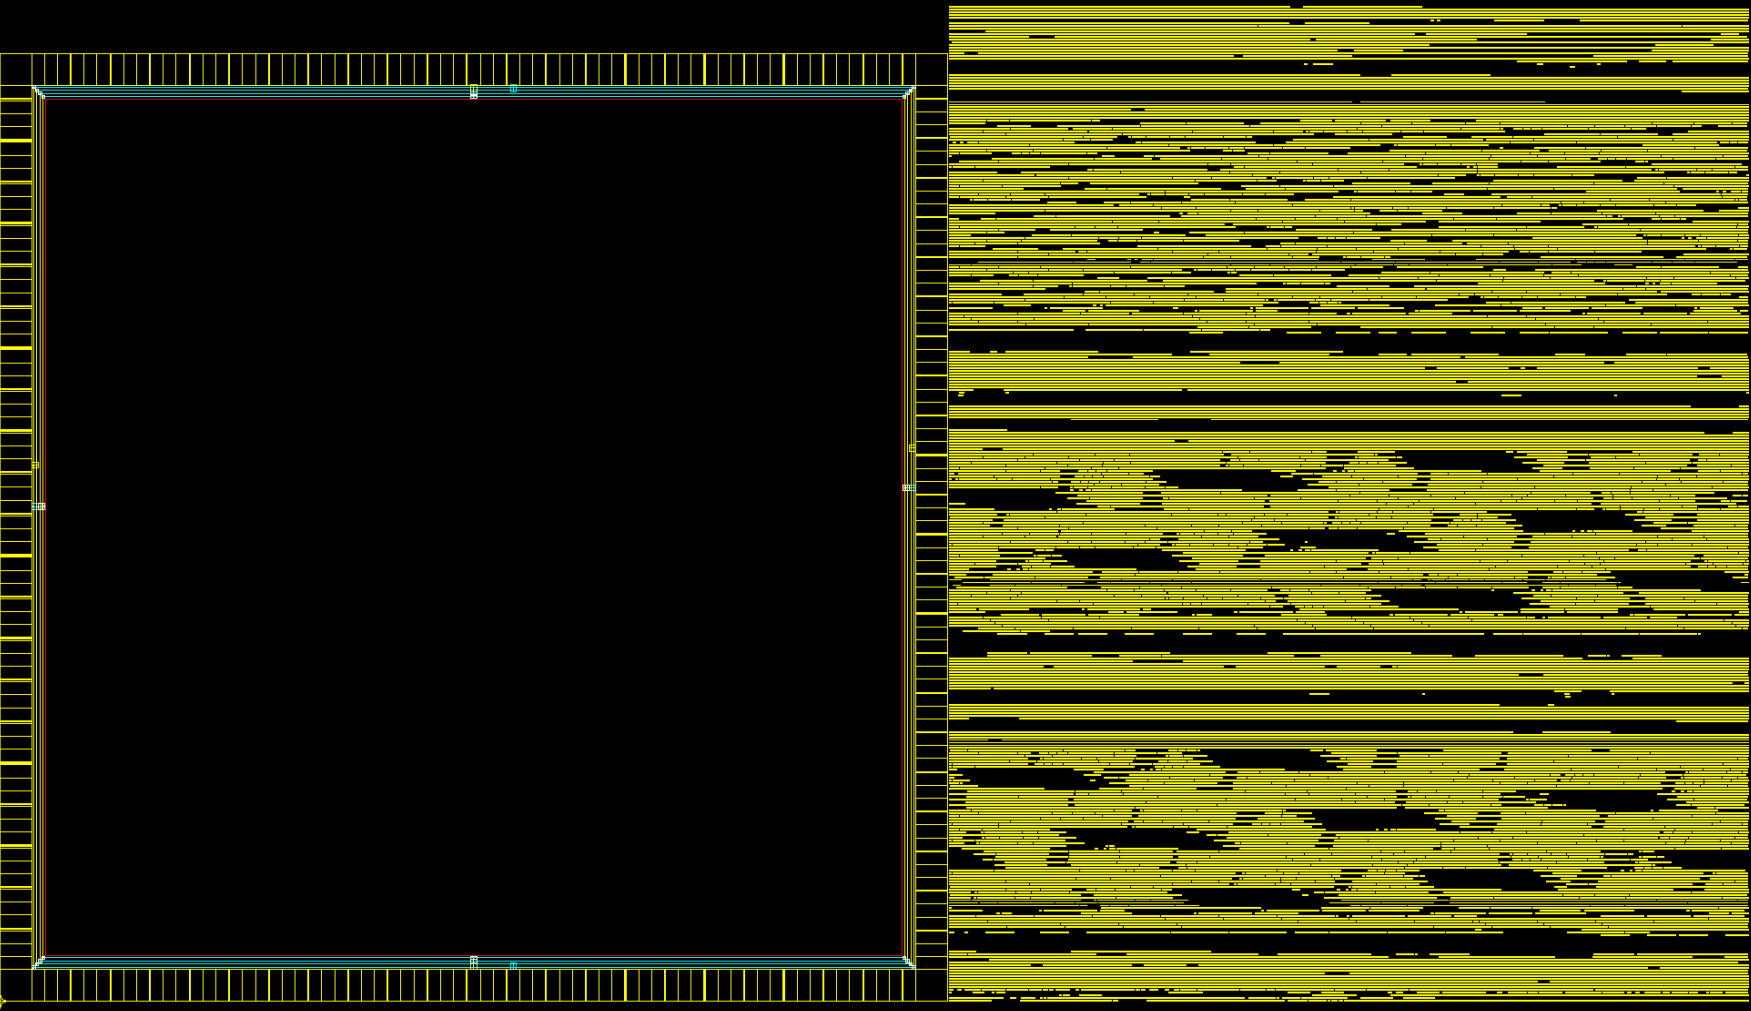
\includegraphics[width =1\textwidth]{figures/astro_floorplan.png}
        \caption{放置 PAD 和电源环后版图}
        \label{astro_floorplan}
    \end{minipage}
    \begin{minipage}{0.45\textwidth}
        \centering
        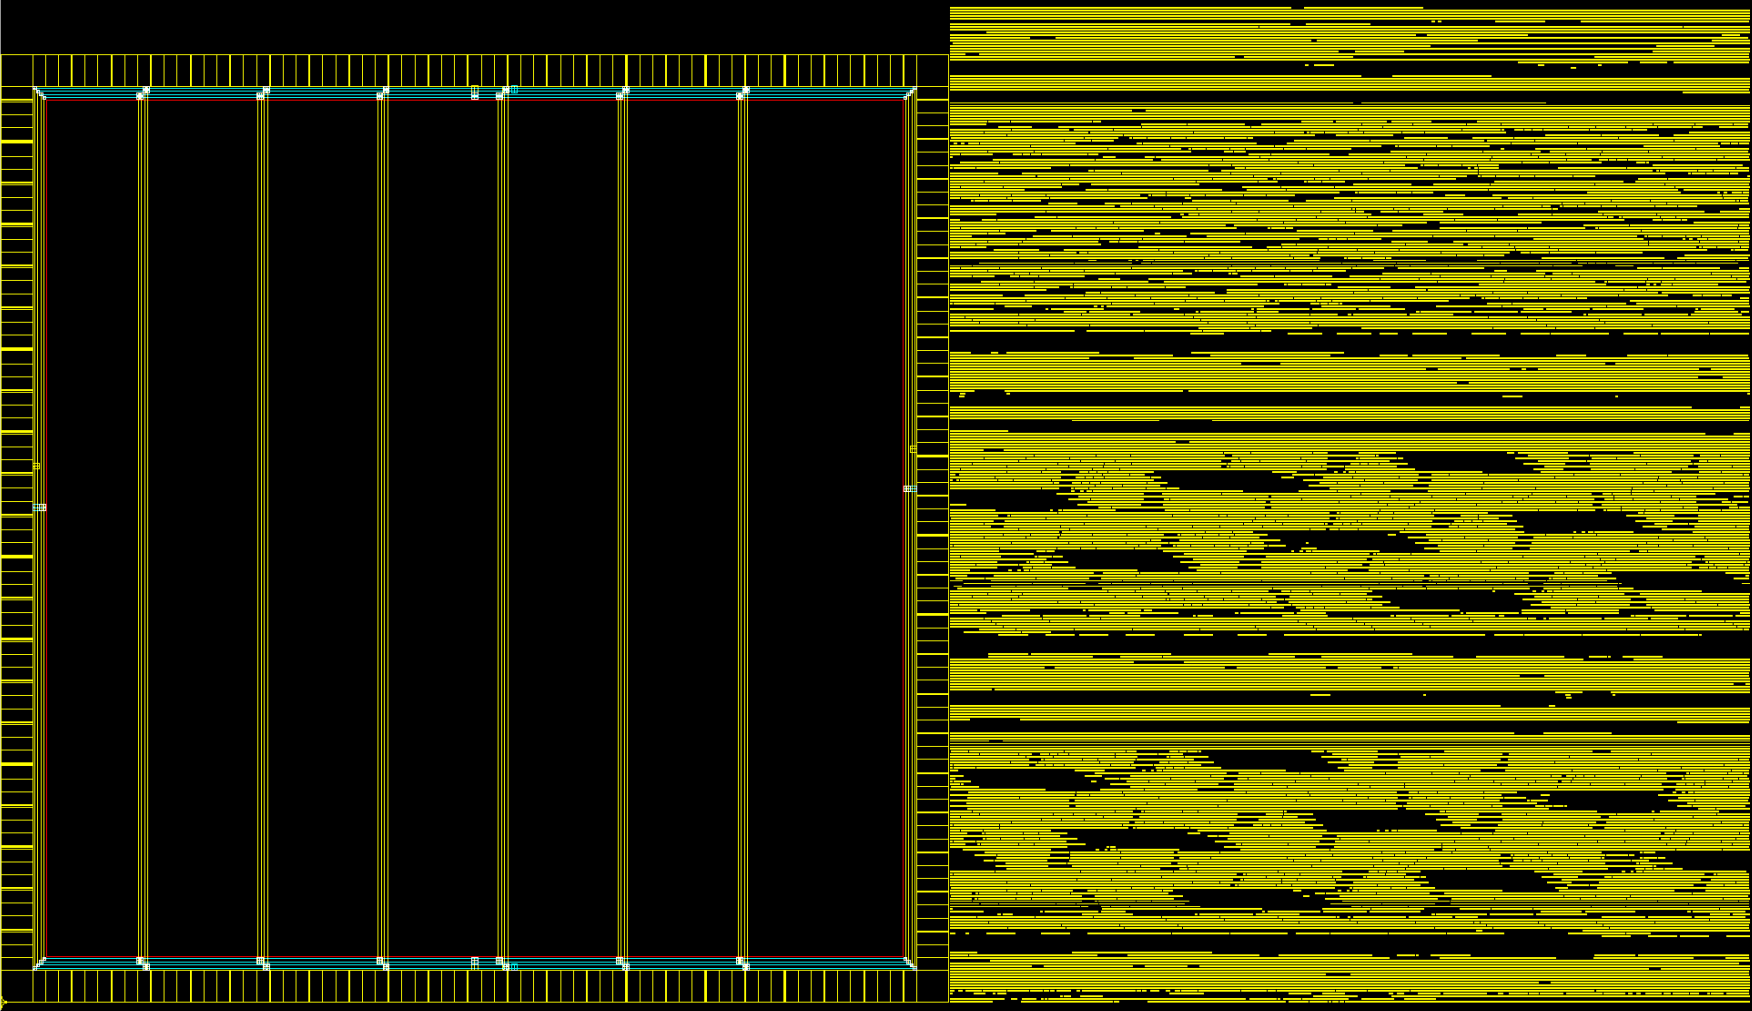
\includegraphics[width =1\textwidth]{figures/astro_floorplan_add_strap.png}
        \caption{添加电源条后版图}
        \label{astro_floorplan_add_strap}
    \end{minipage}
\end{figure}

\subsubsection{规划 stdcell 摆放区域}
设置 blockage 或者直接 cut row,某些电源 PAD 接入的地方,Metal1 很难连接
到电源上,干脆不放 stdcell。另外,电源条下面也不要放上标准单元,
通过 cut row 等方式,把电源条位置闪出来。由于初次规划时未注意,导致在物理验证
 DRC 检查时出现上千个违例,如\autoref{drc_multi_err}所示。与 aes\_asic 设计
对比,大概是因为电源条下面放上标准单元了,如\autoref{drc_multi_err_reason}
所示。

\begin{figure}[htbp]
    \centering
    \begin{minipage}{0.4\textwidth}
        \centering
        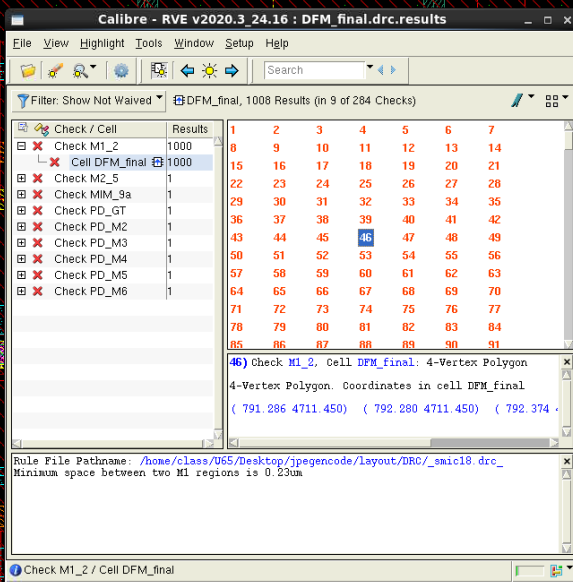
\includegraphics[width =1\textwidth]{figures/drc_multi_err.png}
        \caption{大量 DRC 违例}
        \label{drc_multi_err}
    \end{minipage}
    \quad
    \begin{minipage}{0.45\textwidth}
        \centering
        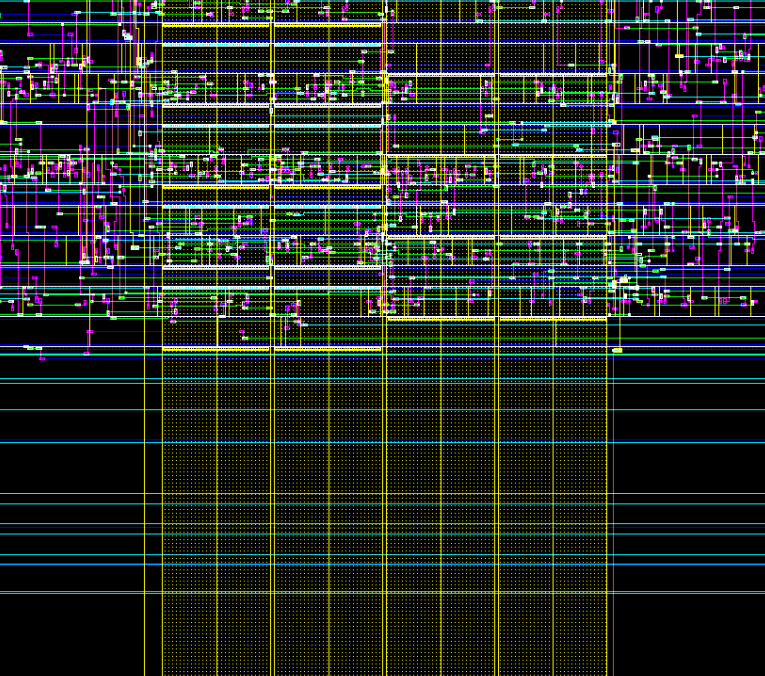
\includegraphics[width =1\textwidth]{figures/drc_multi_err_reason.png}
        \caption{设计的电源条下面存在标准单元}
        \label{drc_multi_err_reason}
    \end{minipage}
\end{figure}

完成后保存 floorplan,floorplan 调整比较麻烦,调整好后保存,下次直接调取脚本。
再次运行时,可以在脚本中使用 \texttt{load "soc\_scripts/row.dump"} 方式加载,
详细步骤可以参考课件。

\subsection{其余步骤}
\subsubsection{时序约束}
Astro 布局布线是 Timing-Driven ,要指定时序约束。DC 时做了时序约束,
是针对 RTL 级的,有较多的高级特性,其他工具未必理解,需要写出较通用的、
门级的 SDC 文件。 

步骤如下:
\begin{enumerate}
    \item 导入 SDC 文件,需要修改 DC 导出的 SDC 文件
    \item Timing Setup,Astro时序分析分阶段,各阶段需要单独设置
    \item 检查约束是否完备
    \item PrePlace Timing Check,此时是比较理想情况的 Timing 检查,一般
    violation 不应该很大,否则需要检查约束或者检查 Design 是否能达到要求。
\end{enumerate}

SDC主要修改的语句有去掉 DC 对“时钟理想化”处理的相关语句、去掉 DC 对工作环境的假设、
增加 \texttt{set\_propagated\_clock [all\_clocks]}。Astro的时序检查分阶段进行,
如布局前的、布局后的,时钟树综合前的、时钟树综合后的,布线前的、布线后的。

\subsubsection{Place}
直接采用Auto place,Astro 的 Place 是 Timing-driven,需要设置 Timing。另外,
要在 Timing Setup 设置工作环境、分析模式等,优化要留余份,检查设置是否符合当前
分析阶段,并设置 Placement Common Options。

\subsubsection{时钟树综合CTS、Post-CTS优化}
进行 CTS,设定时钟树综合约束,最大扇出等信息。然后做 Post-CTS 阶段的 Place。
Place 确定后,做 Post-Place 阶段的时钟树优化。之后检查时序,输出报告。

\subsubsection{Route}
时钟树综合、布局过程中,可能引入一些单元,需要重新连接一次PG网络。
Route 步骤如下:
\begin{enumerate}
    \item 先布时钟线
    \item Timing Setup
    \item Post-Route Opt 及 CTO
    \item Post-Route 时序分析
\end{enumerate}

\subsubsection{DFM}
DFM 一般包括修正天线效应、加 Filler、过孔优化、Fill Notch and Gap、Add Label、
添加 Wire track。

天线效应解决方案有跳线、插入二极管。Astro 所加载的 ANT 规则文件一般应由工艺库中
提供,但若没有提供,可以根据天线效应检查规则文件反推。Astro按规则文件自动修正
天线效应,若规则得当,可修掉大部分,仍可能有部分需要手工处理。添加 Label 是为
 LVS 检查做准备,添加 Wire track 是为了满足后续 DRC 检查中的金属密度规则。

\subsubsection{数据导出}
在数据导出中会先做 LVS ,确认 LVS 没有问题。然后导出网表,用于 LVS、后仿真等,
导出 GDSII 数据,流片数据。导出 SPEF,用于 PT 时序分析。导出 SDF,用于后仿真。

\subsubsection{总结}
其余步骤的脚本内容与 aes\_asic 的相同,不再赘述。仅需修改脚本中设计的文件名,然后
在 \texttt{Astro} 目录下终端执行 \texttt{./soc\_scripts/backend.sh} 即可完成布局布线。
最终布局布线结果如\autoref{astro_layout}所示。

\begin{figure}[htbp]
    \centering
    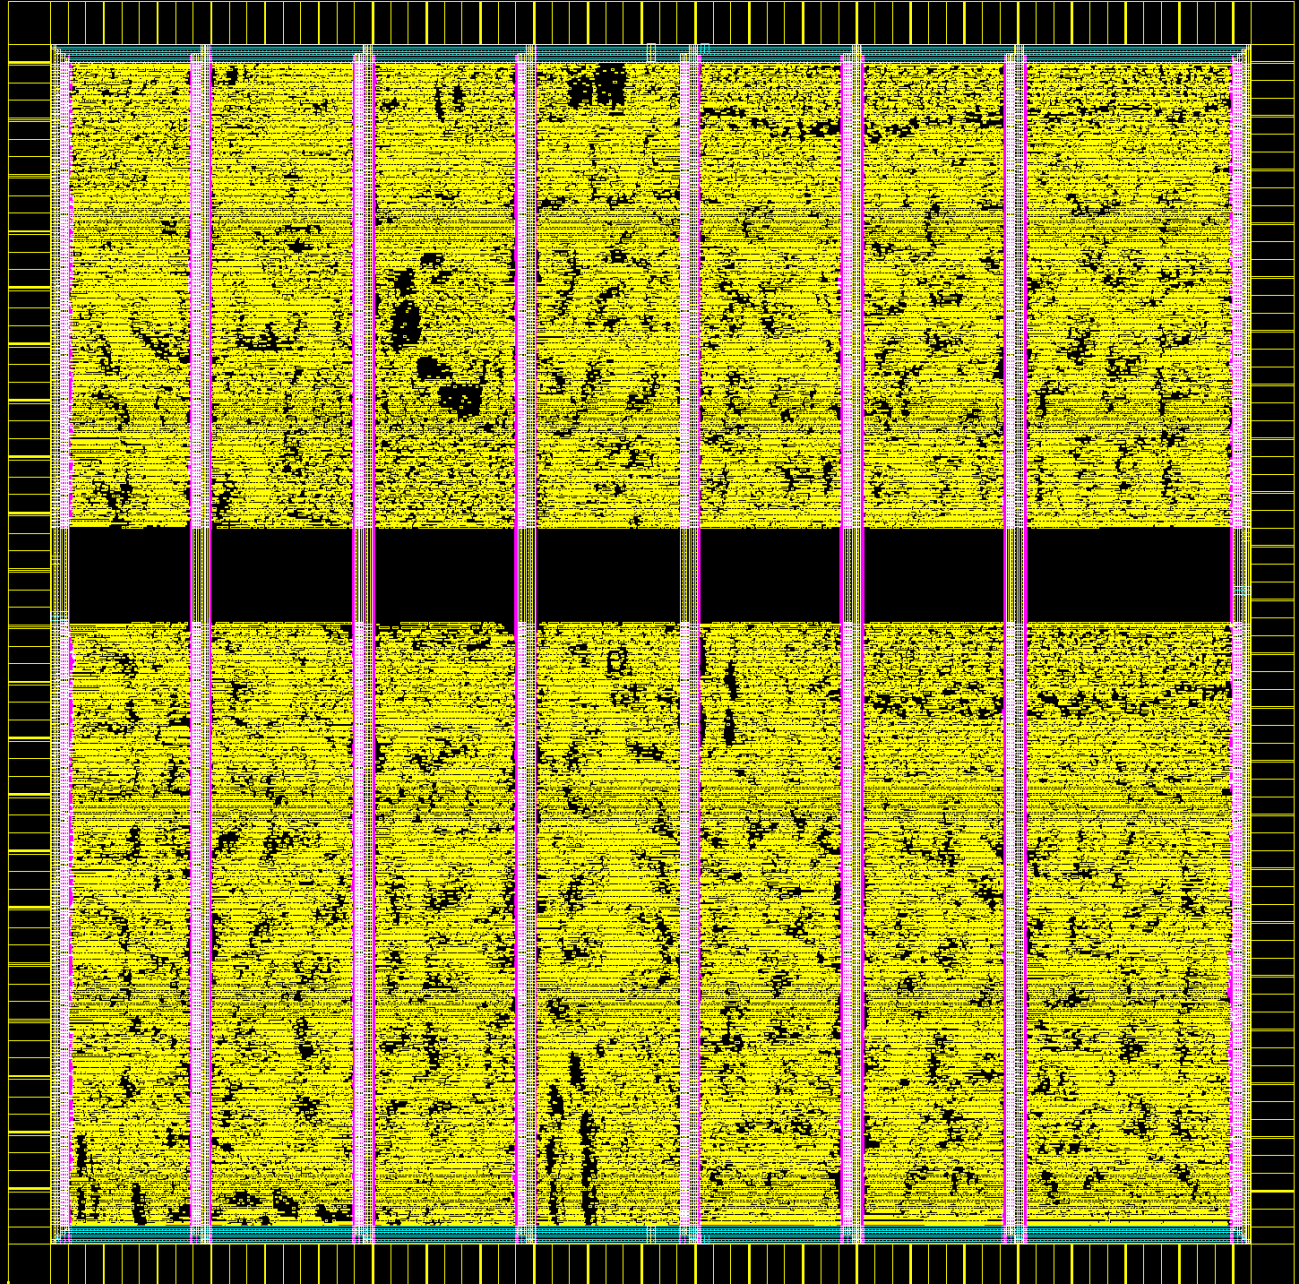
\includegraphics[width =.5\textwidth]{figures/astro_layout.png}
    \caption{Astro 布局布线结果}
    \label{astro_layout}
\end{figure}

\newpage
\section{物理验证}
\subsection{准备 IC5141 环境}
准备工艺库和显示资源,将 \texttt{SmicVTTF\_LO\_SRAM\_MR\_MM\_HV\_LC\_018.tf
display.drf} 复制到 \texttt{layout} 目录。准备基本库,新建 \texttt{cds.lib} 文件,
内容如下所示:
\begin{lstlisting}[style=calibrestyle]
    INCLUDE $CDSHOME/share/cdssetup/cds.lib
    DEFINE SMIC18IOLIB_L_M6 SMIC18IOLIB_L_M6
    DEFINE SMIC18STDLIBM6 SMIC18STDLIBM6
    DEFINE mytools mytools
    DEFINE logo logo
    DEFINE avTech /opt/cadence/assura/tools/assura/etc/avtech/avTech
    DEFINE design_lib_jpeg_asic design_lib_jpeg_asic
\end{lstlisting}

进行快捷键、Calibre配置等的设置,新建 \texttt{.cdsinit} 文件,内容如下:
\begin{lstlisting}[style=calibrestyle]
    load( prependInstallPath( "samples/local/schBindKeys.il" ) )
    load( prependInstallPath( "samples/local/leBindKeys.il" ) )
    load("/opt/mentor/calibre/aoj_cal_2020.3_24.16/lib/calibre.skl")
\end{lstlisting}

\subsubsection{导入库文件}
将 Stdcell、Pad 库以及设计库导入到 IC5141,
本设计导入配置已保存为模板文件,可以直接加载。

\begin{figure}[htbp]
    \centering
    \subfloat[打开导入菜单]{
		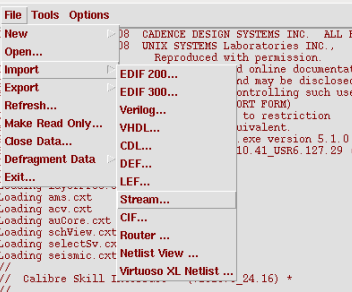
\includegraphics[width=0.3\textwidth]{figures/ic5141stream.png}
	}
    \subfloat[填写配置]{
		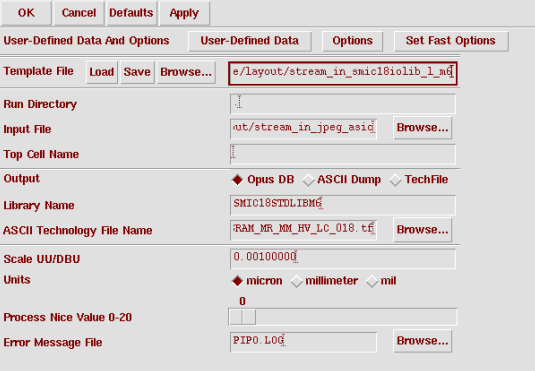
\includegraphics[width=0.32\textwidth]{figures/ic5141_str_config.png}
	}
    \subfloat[导入成功]{
		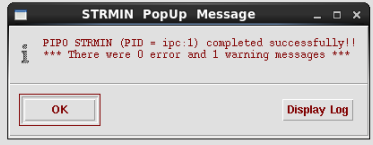
\includegraphics[width=0.31\textwidth]{figures/ic5141_str_suc.png}
	}
    \caption{IC5141 导入库文件}
    \label{ic5141stream}
\end{figure}

\subsection{为电源 PAD 加 Label}
为了进行 LVS,Core 电源 PAD 已加过,只需要为电源 PAD 加 Label。先缩放到某个
 VSSH或VDDH附近,添加 Label,名称分别为 VSSH 、 VDDH。只需要设置一组。
如\autoref{ic5141_add_label}所示。

\begin{figure}[htbp]
    \centering
    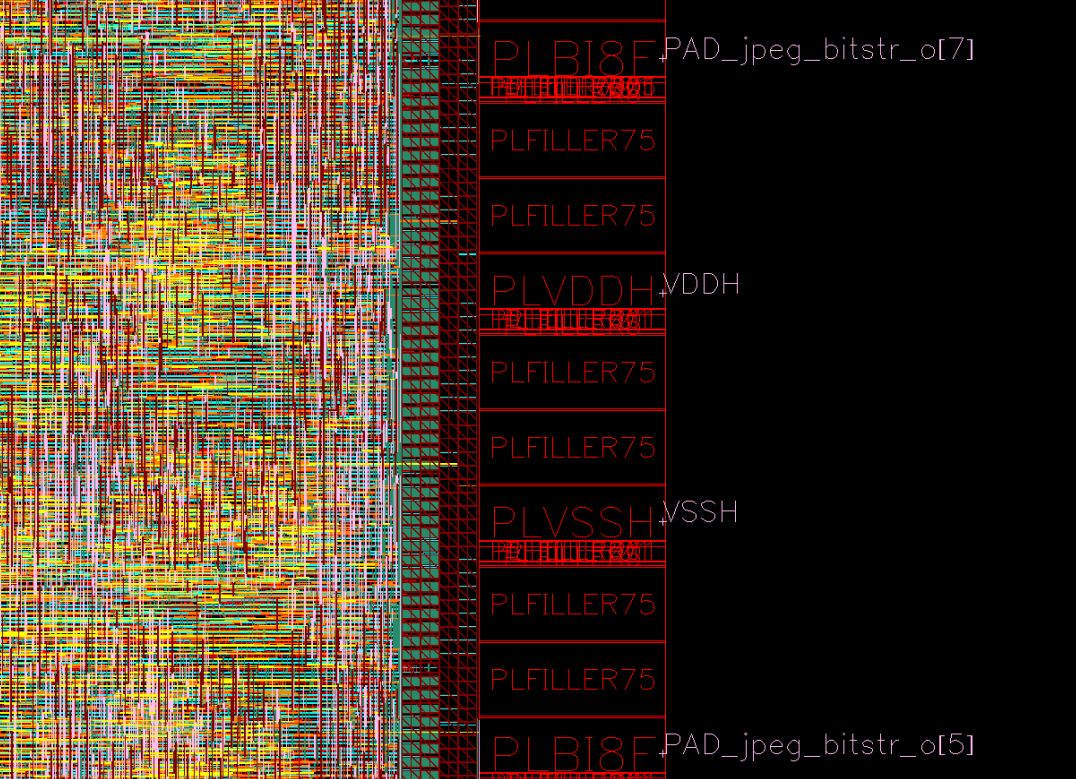
\includegraphics[width =.5\textwidth]{figures/layout_add_label.png}
    \caption{为电源 PAD 加 Label}
    \label{ic5141_add_label}
\end{figure}

\subsection{进行 LVS 检查}
先进行 LVS 检查,确认设计正确。进入 \texttt{layout/LVS} 目录,根据情况
修改 aes\_asic 提供的 \texttt{gen\_spi.sh} 脚本。脚本内容如下:

\begin{lstlisting}[style=bashstyle,name=gen_spi.sh]
    v2lvs -v jpeg_asic.lvs.vg -l smic18.v  -l smic18IO_line.v -s SMIC18IOLIB_L.cdl -s stdcells.cdl -o jpeg_asic.spi -s0 GND -s1 VDD
    echo '.GLOBAL VDDH' >> jpeg_asic.spi
    echo '.GLOBAL VSSH' >> jpeg_asic.spi
\end{lstlisting}

在该目录下终端执行 \texttt{./gen\_spi.sh} ,生成\texttt{.spi}文件。然后在
IC5141 中进行 LVS 检查,按照提示,填写参数,设置规则文件、运行目录等。
Calibre 自动从 IC5141 中提取 layout 数据,并做 LVS 检查,本设计保存了
 runset 文件,可以直接调用。使用中发现,如\autoref{ic5141_lvs}所示,
netlist 处需要每次重填。LVS 检查结果如\autoref{ic5141_lvs_res}所示,
LVS 检查通过。

\begin{figure}[htbp]
    \centering
    \begin{minipage}{0.4\textwidth}
        \centering
        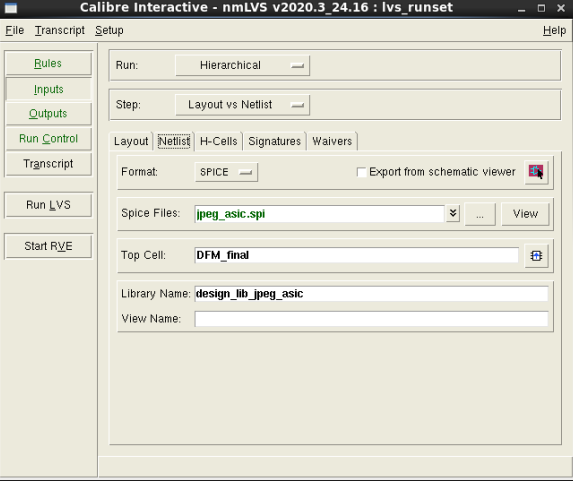
\includegraphics[width =1\textwidth]{figures/lvs_config.png}
        \caption{LVS 检查配置}
        \label{ic5141_lvs}
    \end{minipage}
    \quad
    \begin{minipage}{0.5\textwidth}
        \centering
        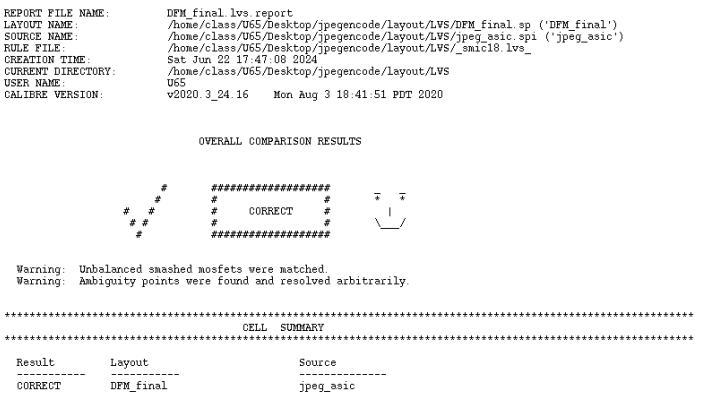
\includegraphics[width =1\textwidth]{figures/lvs_result.png}
        \caption{LVS 检查结果}
        \label{ic5141_lvs_res}
    \end{minipage}
\end{figure}



\subsection{ANT 检查与修正}
ANT 检查要先于 DRC,因为 ANT 修正中可能会引入 DRC 违例,
ANT 检查使用 DRC 菜单调用,但规则文件不同。结果如\autoref{ic5141_ant}所示,
ANT 检查通过。

\begin{figure}[htbp]
    \centering
    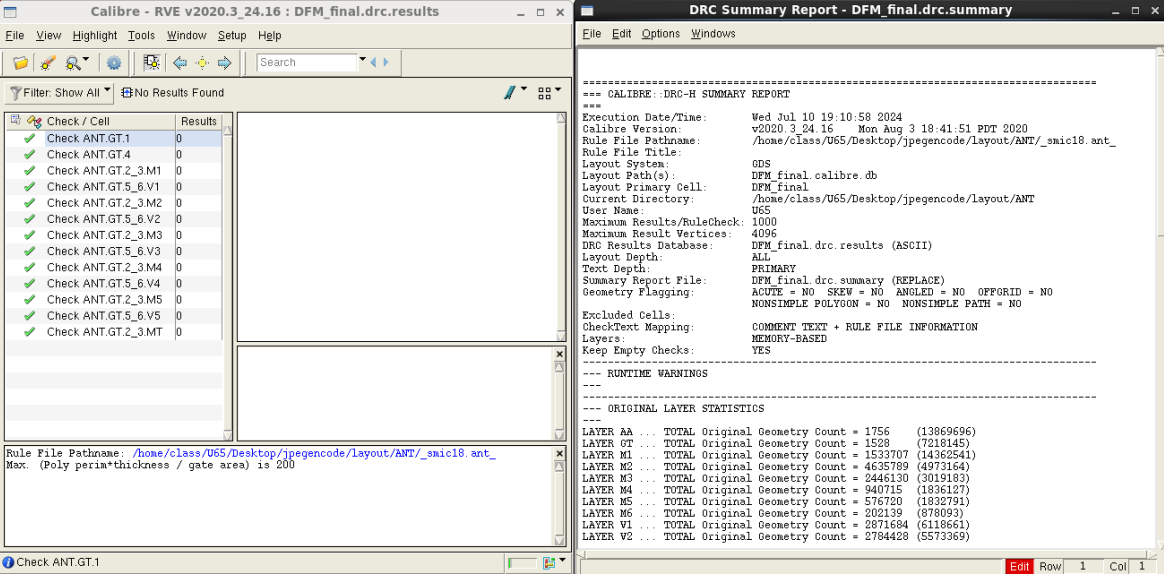
\includegraphics[width =.7\textwidth]{figures/ANT_result.png}
    \caption{ANT 检查结果}
    \label{ic5141_ant}
\end{figure}

\subsection{DRC检查与修正}
DRC 检查也使用 DRC 菜单调用,但规则文件不同。结果如\autoref{ic5141_drc_err}所示。
DRC 大部分通过,出现了较少个数的 DRC 为例,需要进行人工修正。

\begin{figure}[htbp]
    \centering
    \centering
    \subfloat[版图无用连线]{
		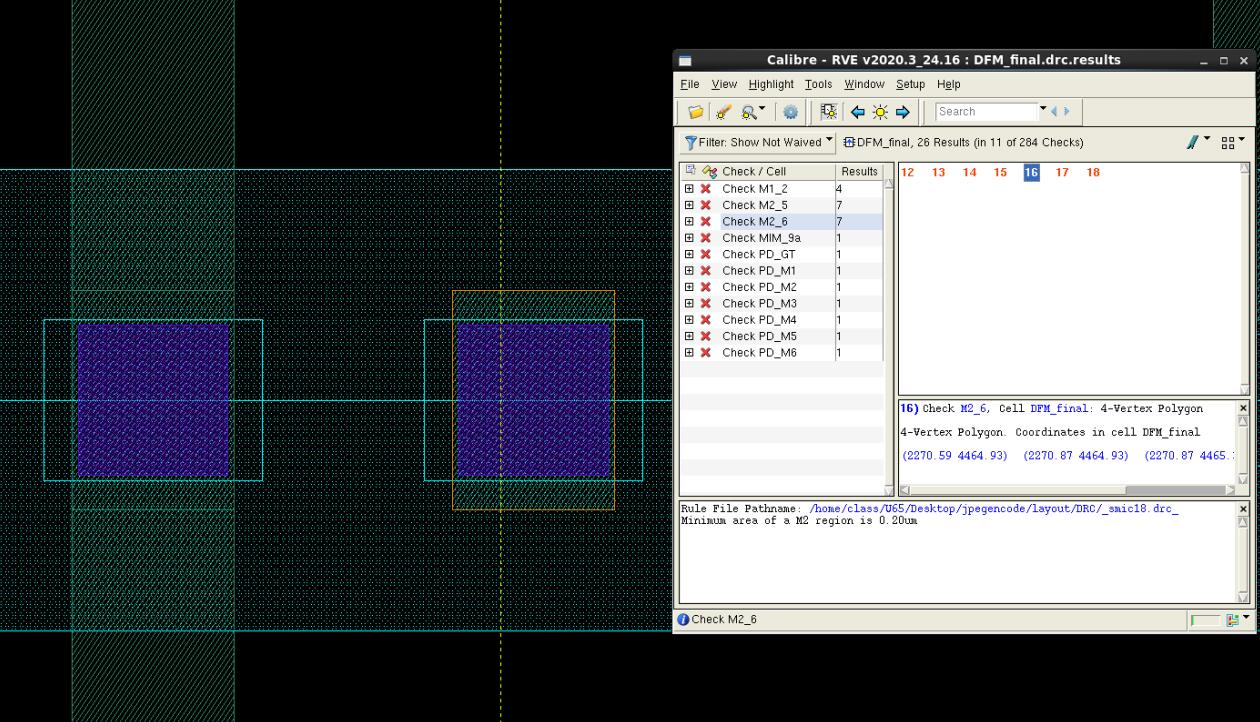
\includegraphics[width=0.53\textwidth]{figures/DRC_del_useless_route.jpg}
        \label{drc_useless_route}
        }
    \subfloat[M1 层缺角]{
		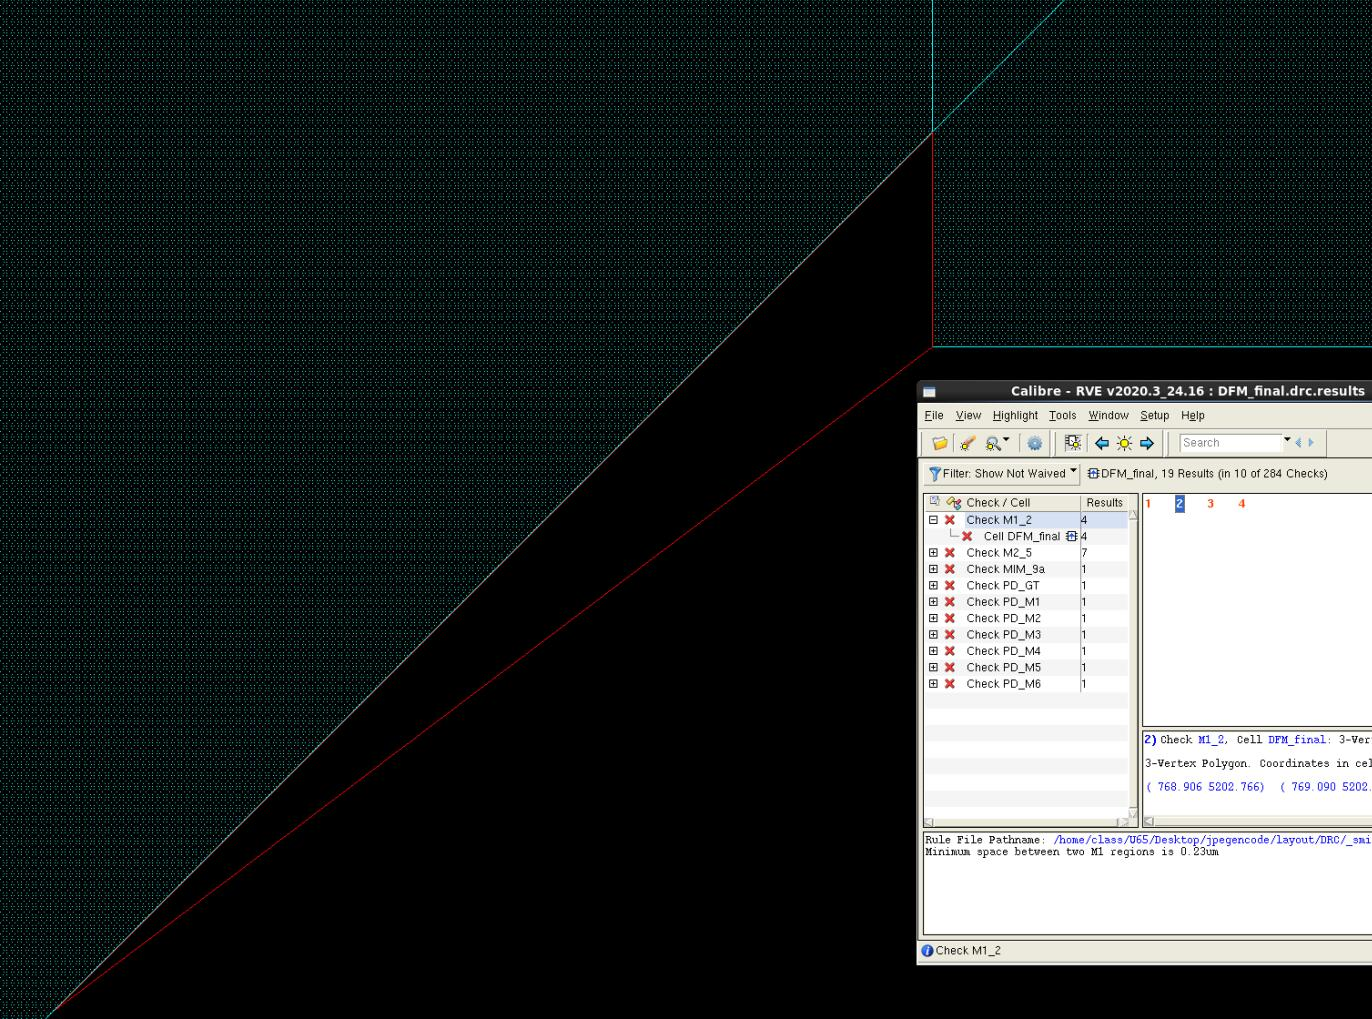
\includegraphics[width=0.43\textwidth]{figures/DRC_fix_angle.jpg}
        \label{drc_fixed_angle}
        }\\
    \subfloat[M2 金属条长度违例]{
		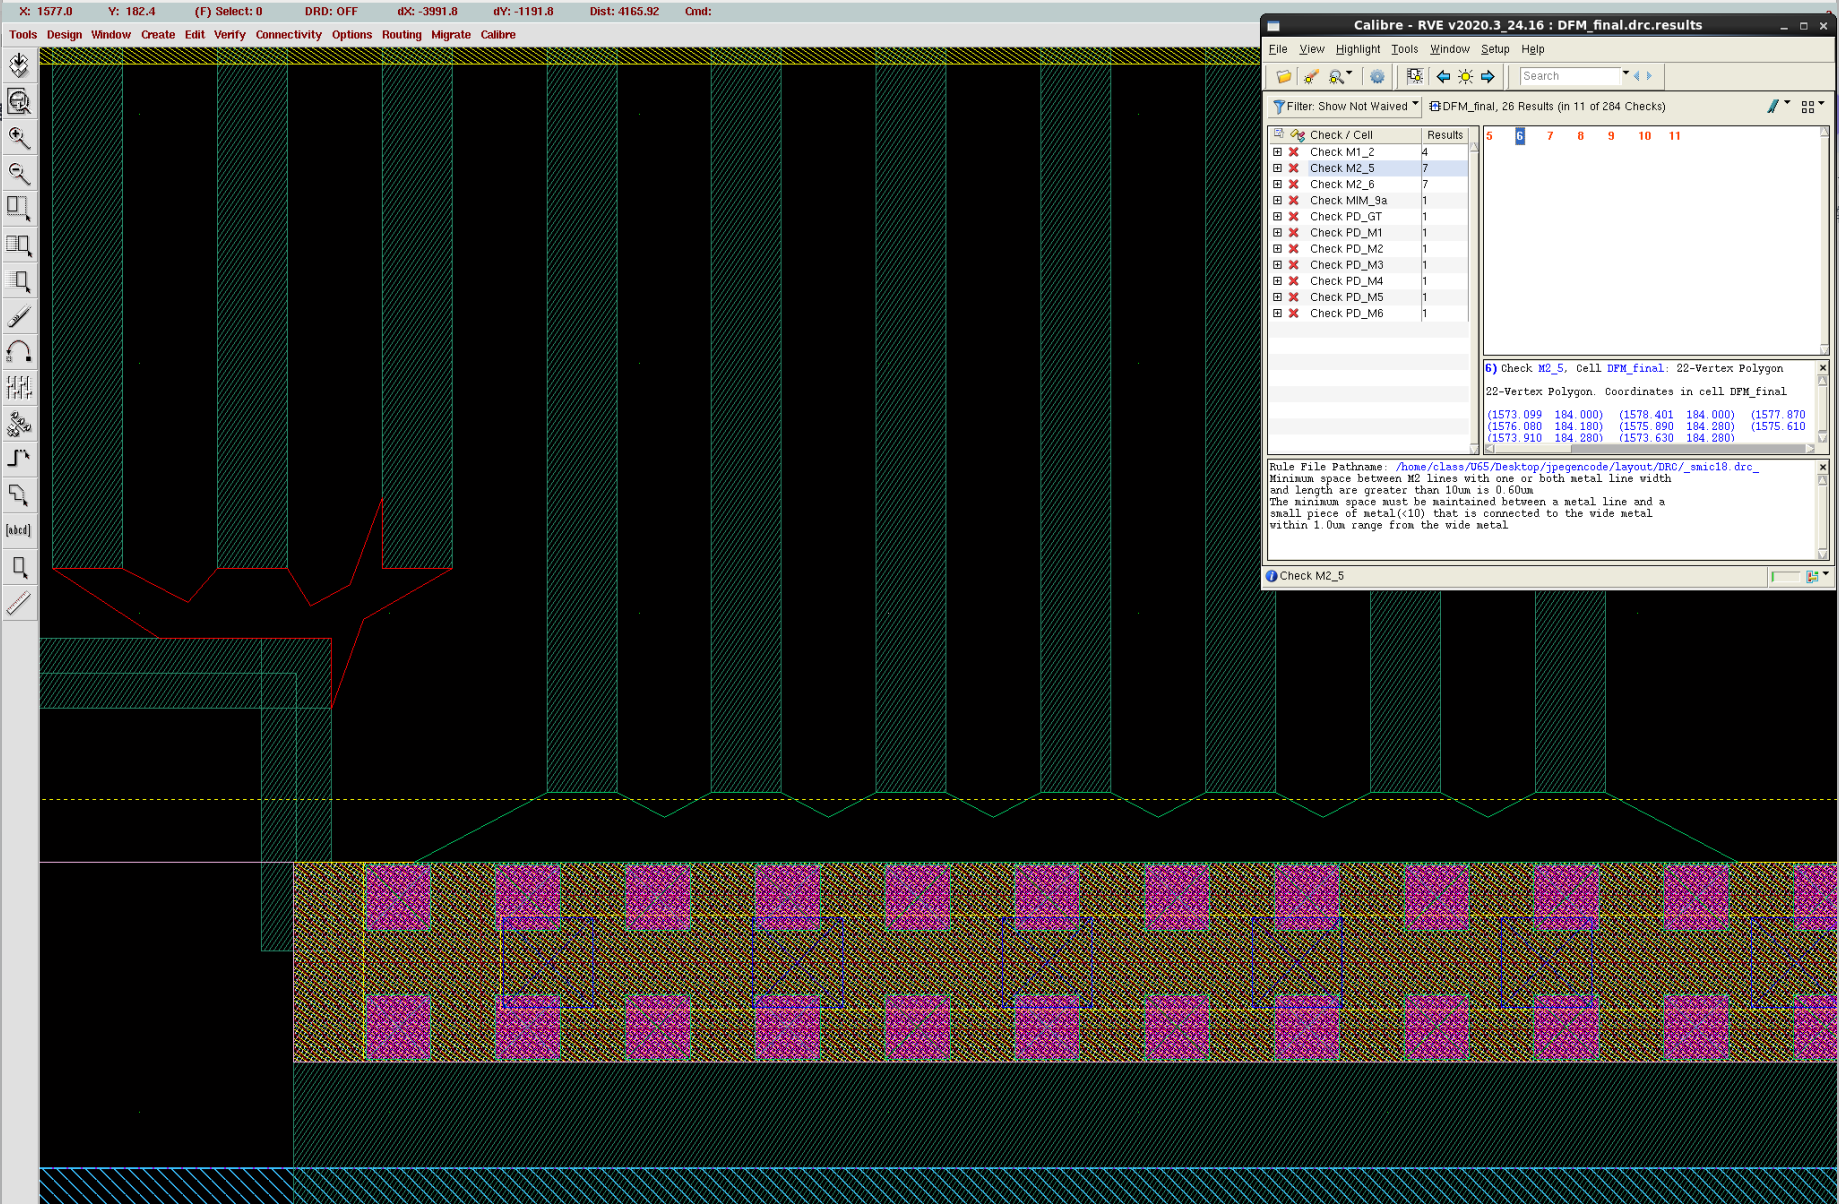
\includegraphics[width=0.48\textwidth]{figures/drc_length_err.png}
        \label{drc_length_err}
        }
    \subfloat[M2 层宽度违例]{
		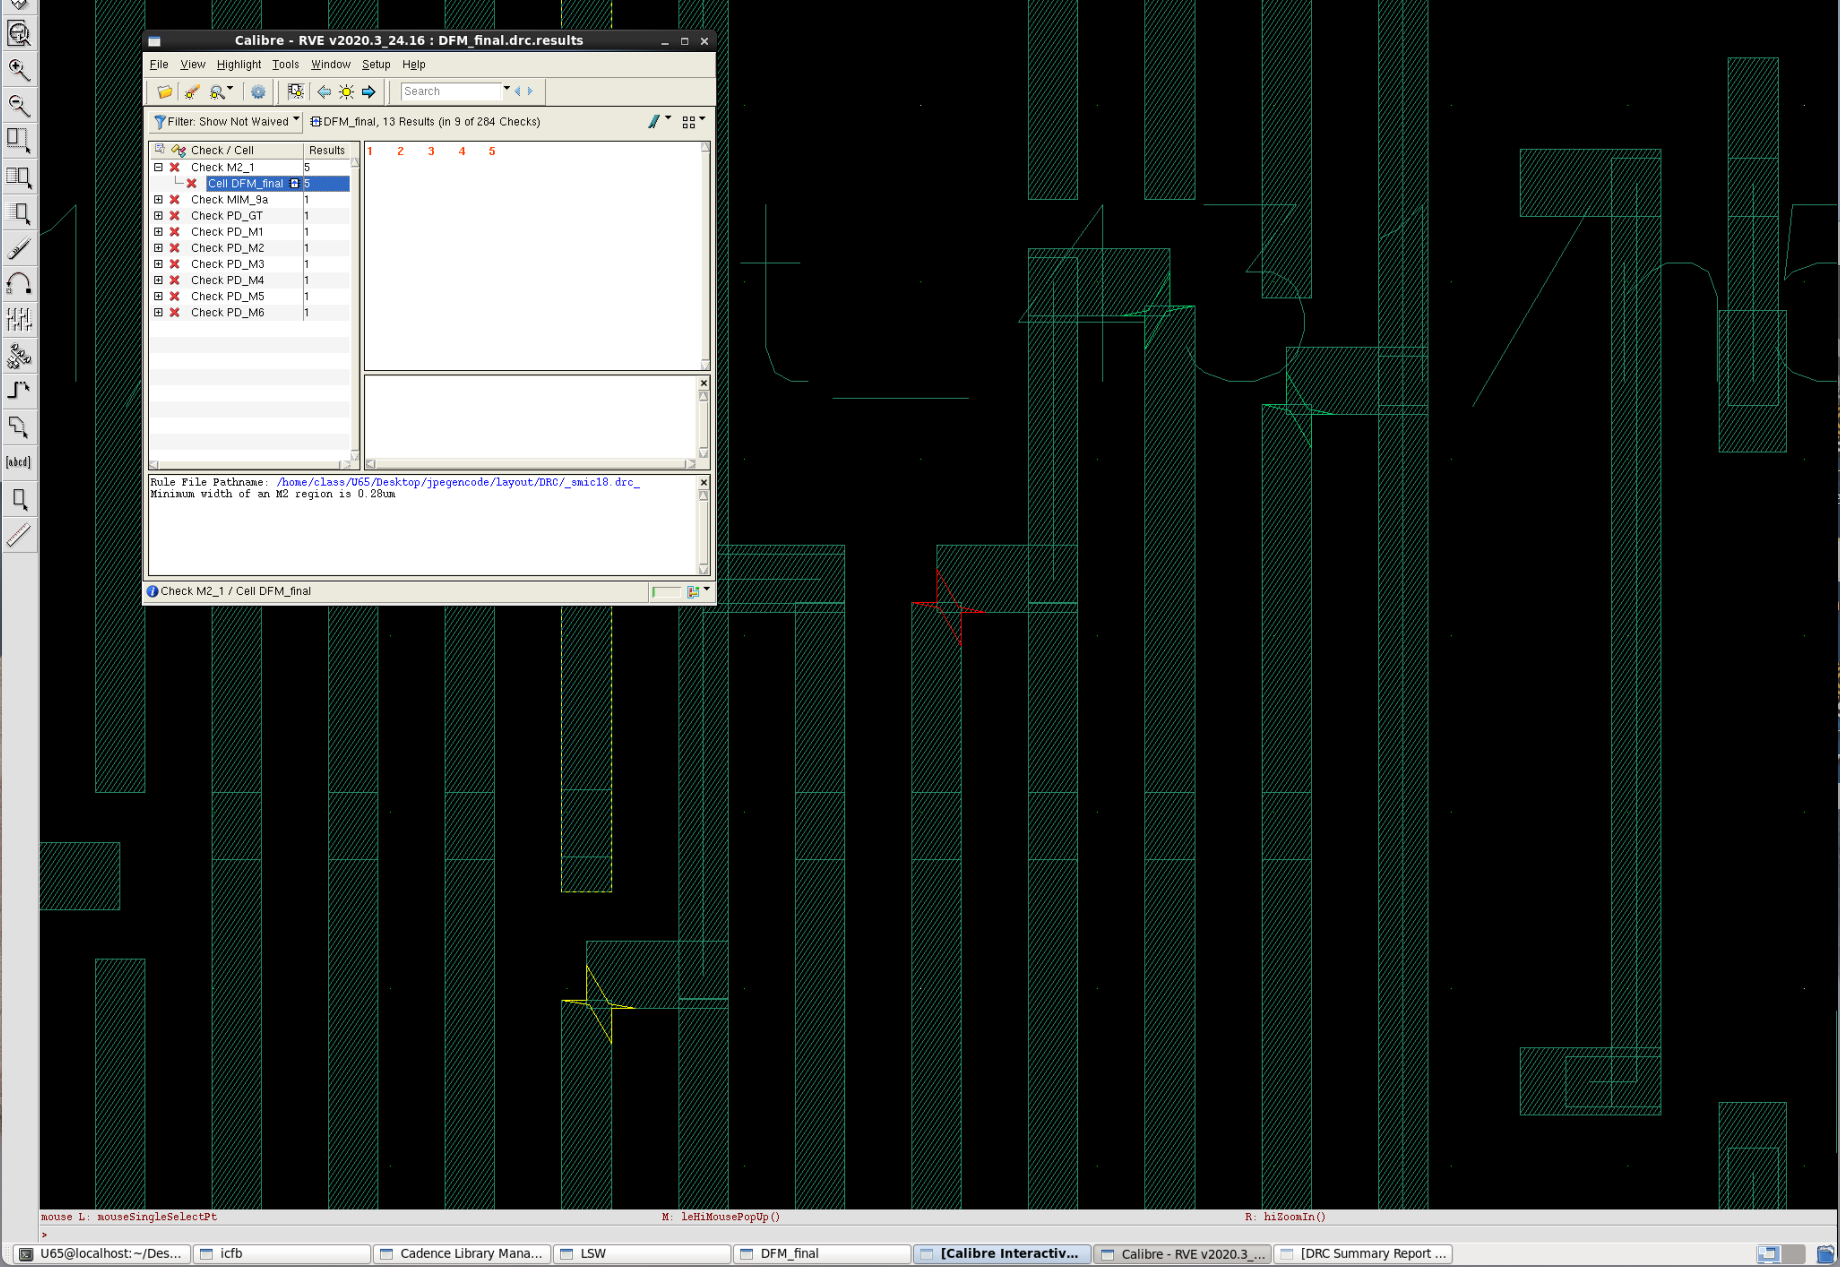
\includegraphics[width=0.47\textwidth]{figures/drc_width_err.png}
        \label{drc_width_err}
        }
    \caption{DRC 检查违例}
    \label{ic5141_drc_err}
\end{figure}

如\autoref{drc_useless_route},该错误为无用连线导致,删除即可。同时进行 LVS 
检查,确保正确。如\autoref{drc_fixed_angle},该错误用 M1 补上缺角即可解决,
一般钝角就可以。\autoref{drc_length_err}的错误修正前检查违例的金属条
有没有上下层连接,没有的话就切短到符合规则,为是 0.6\unit{\um}。\autoref{drc_width_err}
的错误检查对角长度是否够 0.28\unit{\um} ,不够就延迟一段 M2。

修正后再次进行 LVS 检查,ANT 检查,DRC 检查。确保均通过。
DRC 最终结果如\autoref{ic5141_drc_res}所示。其中剩余问题均与密度相关。
这类 DRC 错误暂时可以忽略。

\begin{figure}[htbp]
    \centering
    \begin{minipage}{0.45\textwidth}
        \centering
        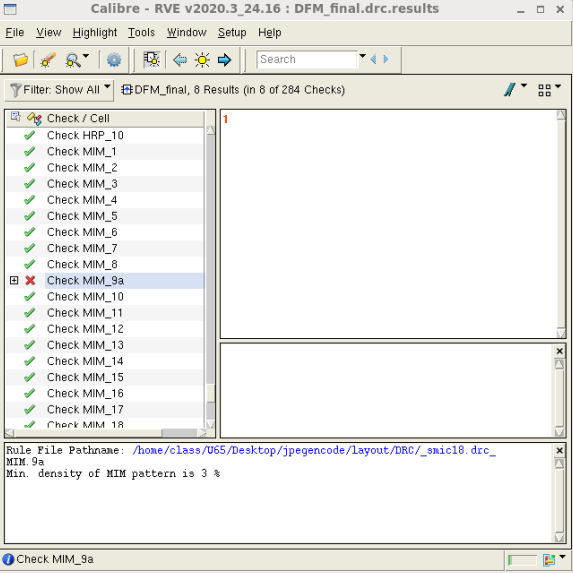
\includegraphics[width =1\textwidth]{figures/drc_results.png}
        \caption{DRC 最终检查结果}
        \label{ic5141_drc_res}
    \end{minipage}
    \quad
    \begin{minipage}{0.45\textwidth}
        \centering
        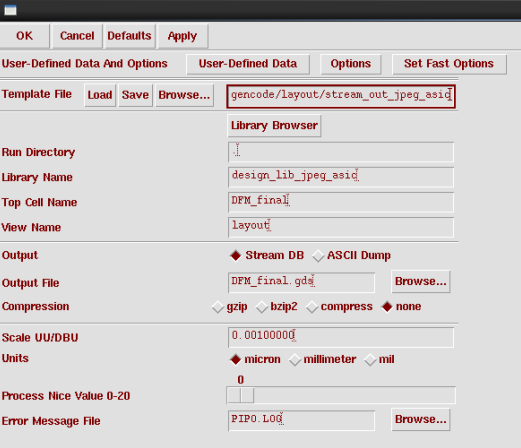
\includegraphics[width =1\textwidth]{figures/ic5141_str_out.png}
        \caption{设计数据导出配置}
        \label{ic5141_str_out}
    \end{minipage}
\end{figure}



\subsection{设计数据导出}
如\autoref{ic5141_str_out}所示配置,导出 GDSII。



\newpage
\section{PT 时序分析}
STA,无需输入激励,电路并不动作(静态含义),分析每一个触发器
的 setup 时间与 hold 时间,即保证在时钟沿采样数据时,数据是有效的。
动态仿真也是确保这一点,下一时钟能得到正确值。动态与静态时序分析比较
STA 无需输入测试向量,覆盖率大。动态仿真只针对特定测试向量,无法证明结果
对所有测试向量都成立;大规模电路,穷举测试向量很困难。STA 缺点是异步电路分析困难
动态时序分析对同步、异步风格电路没有限制。STA 能处理更大设计,所需时间更短
动态仿真缺点是随着设计规模增大,要求时间迅速增长。

PT 使用步骤如下:
\begin{enumerate}
    \item 读入设计
    \item 添加约束
    \item 添加例外
    \item 检查
    \item 分析
\end{enumerate}

\subsection{环境配置}
参照 aes\_asic 设计,确保 \texttt{PT/data\_bend} 指向
 \texttt{../Astro/data\_bend/}。
 
修改 \texttt{PT/.synopsys\_pt.setup} 文件,
内容如下所示:

\begin{lstlisting}[style=tclstyle,name=.synopsys_pt.setup]
    lappend search_path     "/opt/synopsys/pts/P-2019.03/libraries/syn"
\end{lstlisting}

修改 aes\_asic 设计提供的 \texttt{.pt} 文件,并重命名为 \texttt{jpeg\_asic.pt},
内容如下所示:
\begin{lstlisting}[style=tclstyle,name=jpeg_asic.pt]
    set SYS_CLK_PERIOD 20.0
    date
    # Define some variables for design
    set TOP_MODULE		jpeg_asic
    set Rst_list		[list PAD_rst_i ]
    set Clk_list		[list PAD_clk_i ]

    #Read netlist
    read_verilog	data_bend/jpeg_asic.lvs.vg
    current_design $TOP_MODULE
    link_design
\end{lstlisting}
\newpage
\begin{lstlisting}[style=tclstyle,name=jpeg_asic.pt]
    # Define The Design Enviroment
    set_min_library smic18_ss.db -min_version smic18_ff.db
    set_min_library smic18IO_line_ss.db -min_version smic18IO_line_ff.db

    #Read SPEF
    reset_design
    read_parasitics  data_bend/jpeg_asic.spef 

    set_wire_load_mode  "segmented"
    set_wire_load_model -name reference_area_10000000 -library smic18_ss

    # clock defination and reset
    create_clock -name wb_clk -period $SYS_CLK_PERIOD -waveform [list 0 [expr $SYS_CLK_PERIOD /2]]  [get_ports PAD_clk_i]
    set_propagated_clock [all_clocks]

    report_clocks -nosplit >  ${reportsDir}/${TOP_MODULE}.clocks.txt

    # drive and load, max_fanout,max_capacitance
    set MAX_LOAD [load_of smic18_ss/INVHD4X/A]
    set_drive 0	[get_ports "$Rst_list"]
    set_drive 0 	[get_ports "$Clk_list"]
    set_driving_cell -lib_cell INVHD2X [remove_from_collection [all_inputs] \
             [get_ports [list PAD_clk_i PAD_rst_i ]]]
    set_load [expr $MAX_LOAD*3] [all_outputs]
    set_max_fanout 10 [all_inputs]

    # input delay and output delay
    set wb_in_ports [remove_from_collection [all_inputs]  [get_ports [list PAD_clk_i PAD_rst_i]]]
    set wb_out_ports [get_ports [list PAD_jpeg_bitstr_o PAD_dat_rdy_o PAD_eof_bitstr_cnt_o PAD_eof_dat_partial_rdy_o]]

    set_input_delay -max 10 -clock wb_clk $wb_in_ports
    set_input_delay -min 0.1 -clock wb_clk $wb_in_ports

    set_output_delay -max 10 -clock wb_clk $wb_out_ports

\end{lstlisting}
\newpage
\begin{lstlisting}[style=tclstyle,name=jpeg_asic.pt]

    set_output_delay -min -1 -clock wb_clk $wb_out_ports

    # false path
    set_false_path -from [get_ports "$Rst_list"]

    # case_analysis
    set_case_analysis 0 [get_pins "U_rst_i/D"]

    #  Output Reports
    report_design -nosplit >  ${reportsDir}/${TOP_MODULE}.design.txt
    report_port -nosplit >  ${reportsDir}/${TOP_MODULE}.port.txt
    report_net -nosplit >  ${reportsDir}/${TOP_MODULE}.net.txt
    report_constraint -nosplit -all_violators >  ${reportsDir}/${TOP_MODULE}.constraint.txt
    report_timing -nosplit >  ${reportsDir}/${TOP_MODULE}.timing.txt

    #  Output Results
    write_sdf  data_bend/${TOP_MODULE}_post_APR.PT.sdf

    date
    exit
\end{lstlisting}

然后对 \texttt{run\_pt.sh} 修改,如下所示:
\begin{lstlisting}[style=bashstyle,name=run_fm.scr]
    #!/bin/bash
    mkdir -p logs
    mkdir -p reports
    pt_shell -f jpeg_asic.pt |tee -i logs/jpeg_asic.pt.log
\end{lstlisting}

在 \texttt{PT} 目录下终端执行 \texttt{./run\_pt.sh},执行结果
如\autoref{pt_res}所示。

\begin{figure}[htbp]
    \centering
    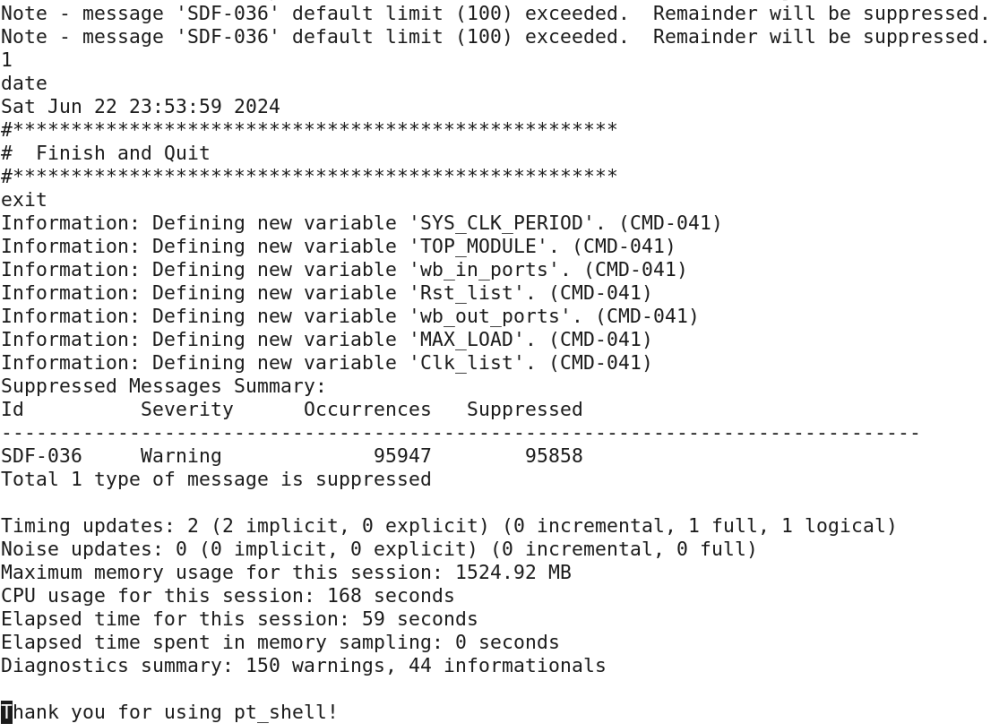
\includegraphics[width =.7\textwidth]{figures/pt_results.png}
    \caption{PT 脚本执行输出}
    \label{pt_res}
\end{figure}

\subsection{查看报告}
PT 时序分析报告输出到 \texttt{PT/reports} 目录下,其中时序报告如\autoref{pt_timing}所示。

\begin{figure}[htbp]
    \centering
    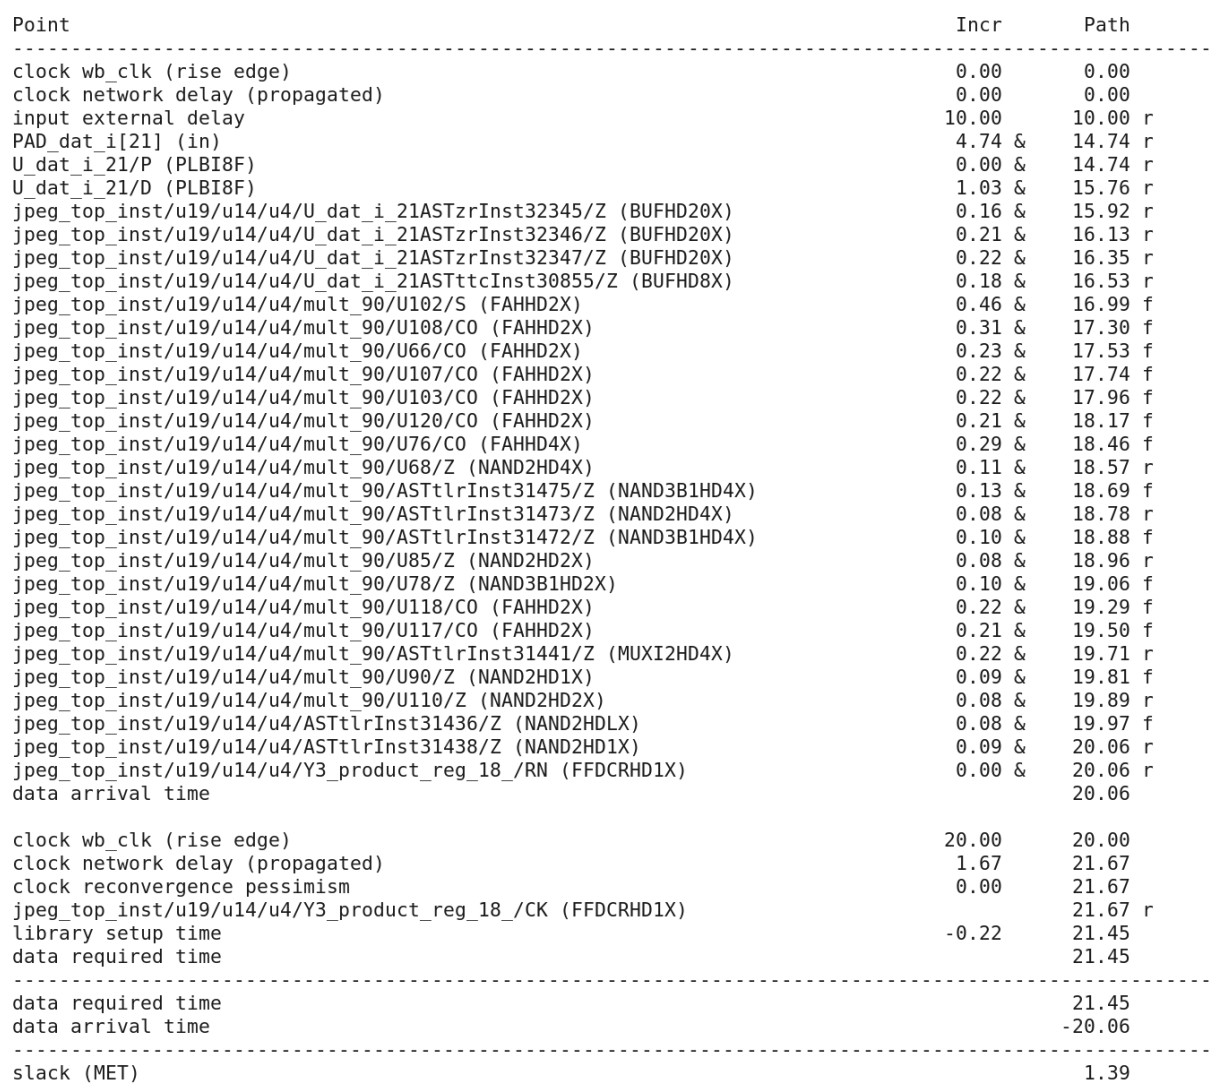
\includegraphics[width =.7\textwidth]{figures/pt_timing.png}
    \caption{PT 时序分析报告}
    \label{pt_timing}
\end{figure}

由图可知, data required time 为 21.45\unit{\ns}, data arrival time 
为 -20.06\unit{\ns},slack 为 1.39\unit{\ns}。满足时序约束。



\newpage
\section{设计心得}
在本次数字集成电路设计课程设计中,我选择了已有设计 jpegencode,
该设计可以将 TIF 格式图像转换为 JPEG 格式。整个设计过程中,
我完成了以下任务:RTL 级仿真、DC 综合、FM 形式验证,以及课程要求的可选部分:
Astro 自动布局布线、后端版图验证、PT 时序分析。

在 RTL 级仿真阶段,我使用了自写的仿真脚本并借助 Questasim 工具完成了仿真工作。
仿真脚本的编写使我深入理解了设计的各个模块和其交互方式。DC 综合使用
了 SMIC18 工艺库进行。并按照要求设置了约束。综合完成后,我详细检查了时序报告,
分析了最差时序路径。通过这些分析,我了解到设计在实际运行时可能遇到的瓶颈。

Astro 自动布局布线阶段,我遇到了一些困难。在老师的帮助下,我逐步解决了这些问题,
成功完成了后端物理验证。这个过程让我认识到,后端设计不仅需要扎实的理论基础,
还需要耐心和细致的实践操作。PT 时序分析阶段,我重点关注了设计的时序约束,
通过详细的时序分析,确保了设计的时序稳定性。

在整个项目进行过程中,我使用了 Git 进行版本控制。
这不仅帮助我有效地管理了代码版本,还让我在遇到问题时能够快速回溯到
之前的稳定版本。在此过程中,我也学到了许多关于版本控制的知识和技巧。

这次课程设计不仅让我掌握了数字集成电路设计的基本流程和工具使用方法,
还让我深刻体会到实践操作的重要性。每一个环节的设计和验证,都需要仔细的思考
和不断的尝试。在这个过程中,我也学会了如何有效地利用工具和资源,解决实际设计
中的问题。这次课程设计让我在理论知识和实践技能方面都有了很大的提升,
也让我对数字集成电路设计有了更深入的理解和更强的兴趣。未来,
我将继续深入学习和实践,争取在这一领域取得更大的进步。

%%----------- 参考文献 -------------------%%
%在reference.bib文件中填写参考文献,此处自动生成
% \phantomsection
% \addcontentsline{toc}{section}{参考文献} 
% \reference


\end{document}